% Options for packages loaded elsewhere
\PassOptionsToPackage{unicode}{hyperref}
\PassOptionsToPackage{hyphens}{url}
%
\documentclass[
]{article}
\usepackage{amsmath,amssymb}
\usepackage{lmodern}
\usepackage{ifxetex,ifluatex}
\ifnum 0\ifxetex 1\fi\ifluatex 1\fi=0 % if pdftex
  \usepackage[T1]{fontenc}
  \usepackage[utf8]{inputenc}
  \usepackage{textcomp} % provide euro and other symbols
\else % if luatex or xetex
  \usepackage{unicode-math}
  \defaultfontfeatures{Scale=MatchLowercase}
  \defaultfontfeatures[\rmfamily]{Ligatures=TeX,Scale=1}
\fi
% Use upquote if available, for straight quotes in verbatim environments
\IfFileExists{upquote.sty}{\usepackage{upquote}}{}
\IfFileExists{microtype.sty}{% use microtype if available
  \usepackage[]{microtype}
  \UseMicrotypeSet[protrusion]{basicmath} % disable protrusion for tt fonts
}{}
\makeatletter
\@ifundefined{KOMAClassName}{% if non-KOMA class
  \IfFileExists{parskip.sty}{%
    \usepackage{parskip}
  }{% else
    \setlength{\parindent}{0pt}
    \setlength{\parskip}{6pt plus 2pt minus 1pt}}
}{% if KOMA class
  \KOMAoptions{parskip=half}}
\makeatother
\usepackage{xcolor}
\IfFileExists{xurl.sty}{\usepackage{xurl}}{} % add URL line breaks if available
\IfFileExists{bookmark.sty}{\usepackage{bookmark}}{\usepackage{hyperref}}
\hypersetup{
  pdftitle={Intro to tidymodels},
  pdfauthor={Author: Steve Pittard wsp@emory.edu},
  hidelinks,
  pdfcreator={LaTeX via pandoc}}
\urlstyle{same} % disable monospaced font for URLs
\usepackage[margin=1in]{geometry}
\usepackage{color}
\usepackage{fancyvrb}
\newcommand{\VerbBar}{|}
\newcommand{\VERB}{\Verb[commandchars=\\\{\}]}
\DefineVerbatimEnvironment{Highlighting}{Verbatim}{commandchars=\\\{\}}
% Add ',fontsize=\small' for more characters per line
\usepackage{framed}
\definecolor{shadecolor}{RGB}{248,248,248}
\newenvironment{Shaded}{\begin{snugshade}}{\end{snugshade}}
\newcommand{\AlertTok}[1]{\textcolor[rgb]{0.94,0.16,0.16}{#1}}
\newcommand{\AnnotationTok}[1]{\textcolor[rgb]{0.56,0.35,0.01}{\textbf{\textit{#1}}}}
\newcommand{\AttributeTok}[1]{\textcolor[rgb]{0.77,0.63,0.00}{#1}}
\newcommand{\BaseNTok}[1]{\textcolor[rgb]{0.00,0.00,0.81}{#1}}
\newcommand{\BuiltInTok}[1]{#1}
\newcommand{\CharTok}[1]{\textcolor[rgb]{0.31,0.60,0.02}{#1}}
\newcommand{\CommentTok}[1]{\textcolor[rgb]{0.56,0.35,0.01}{\textit{#1}}}
\newcommand{\CommentVarTok}[1]{\textcolor[rgb]{0.56,0.35,0.01}{\textbf{\textit{#1}}}}
\newcommand{\ConstantTok}[1]{\textcolor[rgb]{0.00,0.00,0.00}{#1}}
\newcommand{\ControlFlowTok}[1]{\textcolor[rgb]{0.13,0.29,0.53}{\textbf{#1}}}
\newcommand{\DataTypeTok}[1]{\textcolor[rgb]{0.13,0.29,0.53}{#1}}
\newcommand{\DecValTok}[1]{\textcolor[rgb]{0.00,0.00,0.81}{#1}}
\newcommand{\DocumentationTok}[1]{\textcolor[rgb]{0.56,0.35,0.01}{\textbf{\textit{#1}}}}
\newcommand{\ErrorTok}[1]{\textcolor[rgb]{0.64,0.00,0.00}{\textbf{#1}}}
\newcommand{\ExtensionTok}[1]{#1}
\newcommand{\FloatTok}[1]{\textcolor[rgb]{0.00,0.00,0.81}{#1}}
\newcommand{\FunctionTok}[1]{\textcolor[rgb]{0.00,0.00,0.00}{#1}}
\newcommand{\ImportTok}[1]{#1}
\newcommand{\InformationTok}[1]{\textcolor[rgb]{0.56,0.35,0.01}{\textbf{\textit{#1}}}}
\newcommand{\KeywordTok}[1]{\textcolor[rgb]{0.13,0.29,0.53}{\textbf{#1}}}
\newcommand{\NormalTok}[1]{#1}
\newcommand{\OperatorTok}[1]{\textcolor[rgb]{0.81,0.36,0.00}{\textbf{#1}}}
\newcommand{\OtherTok}[1]{\textcolor[rgb]{0.56,0.35,0.01}{#1}}
\newcommand{\PreprocessorTok}[1]{\textcolor[rgb]{0.56,0.35,0.01}{\textit{#1}}}
\newcommand{\RegionMarkerTok}[1]{#1}
\newcommand{\SpecialCharTok}[1]{\textcolor[rgb]{0.00,0.00,0.00}{#1}}
\newcommand{\SpecialStringTok}[1]{\textcolor[rgb]{0.31,0.60,0.02}{#1}}
\newcommand{\StringTok}[1]{\textcolor[rgb]{0.31,0.60,0.02}{#1}}
\newcommand{\VariableTok}[1]{\textcolor[rgb]{0.00,0.00,0.00}{#1}}
\newcommand{\VerbatimStringTok}[1]{\textcolor[rgb]{0.31,0.60,0.02}{#1}}
\newcommand{\WarningTok}[1]{\textcolor[rgb]{0.56,0.35,0.01}{\textbf{\textit{#1}}}}
\usepackage{longtable,booktabs,array}
\usepackage{calc} % for calculating minipage widths
% Correct order of tables after \paragraph or \subparagraph
\usepackage{etoolbox}
\makeatletter
\patchcmd\longtable{\par}{\if@noskipsec\mbox{}\fi\par}{}{}
\makeatother
% Allow footnotes in longtable head/foot
\IfFileExists{footnotehyper.sty}{\usepackage{footnotehyper}}{\usepackage{footnote}}
\makesavenoteenv{longtable}
\usepackage{graphicx}
\makeatletter
\def\maxwidth{\ifdim\Gin@nat@width>\linewidth\linewidth\else\Gin@nat@width\fi}
\def\maxheight{\ifdim\Gin@nat@height>\textheight\textheight\else\Gin@nat@height\fi}
\makeatother
% Scale images if necessary, so that they will not overflow the page
% margins by default, and it is still possible to overwrite the defaults
% using explicit options in \includegraphics[width, height, ...]{}
\setkeys{Gin}{width=\maxwidth,height=\maxheight,keepaspectratio}
% Set default figure placement to htbp
\makeatletter
\def\fps@figure{htbp}
\makeatother
\setlength{\emergencystretch}{3em} % prevent overfull lines
\providecommand{\tightlist}{%
  \setlength{\itemsep}{0pt}\setlength{\parskip}{0pt}}
\setcounter{secnumdepth}{-\maxdimen} % remove section numbering
\ifluatex
  \usepackage{selnolig}  % disable illegal ligatures
\fi

\title{Intro to tidymodels}
\author{Author: Steve Pittard
\href{mailto:wsp@emory.edu}{\nolinkurl{wsp@emory.edu}}}
\date{Last update: 14 Oct 2021}

\begin{document}
\maketitle

Note you may use this in your work as long as it's not part of a
commerical project. Any use should cite this notebook and author
accordingly.

\begin{Shaded}
\begin{Highlighting}[]
\NormalTok{https}\SpecialCharTok{:}\ErrorTok{//}\NormalTok{cimentadaj.github.io}\SpecialCharTok{/}\NormalTok{blog}\SpecialCharTok{/}\DecValTok{2020{-}02{-}06}\SpecialCharTok{{-}}\NormalTok{the}\SpecialCharTok{{-}}\NormalTok{simplest}\SpecialCharTok{{-}}\NormalTok{tidy}\SpecialCharTok{{-}}\NormalTok{machine}\SpecialCharTok{{-}}\NormalTok{learning}\SpecialCharTok{{-}}\NormalTok{workflow}\SpecialCharTok{/}\NormalTok{the}\SpecialCharTok{{-}}\NormalTok{simplest}\SpecialCharTok{{-}}\NormalTok{tidy}\SpecialCharTok{{-}}\NormalTok{machine}\SpecialCharTok{{-}}\NormalTok{learning}\SpecialCharTok{{-}}\NormalTok{workflow}\SpecialCharTok{/}
\end{Highlighting}
\end{Shaded}

\hypertarget{introduction}{%
\section{Introduction}\label{introduction}}

This notebook motivates the use of the tidy models as a way to simplify
the processes associated with building models and evaluating them. While
it is entirely possible to use Base R methods to organize data and build
models thereon, the tidyverse and tidymodels provide a uniform interface
for interacting with data and model assembly.

What I hope you get out of this includes the following:

\begin{enumerate}
\def\labelenumi{\arabic{enumi})}
\tightlist
\item
  An idea of what is involved into basic ML and building models
\item
  You can use Base R to do modeling and it's fine
\item
  But the tidyverse offers a well thought out philosophy for managing
  data
\item
  The tidymodels package builds on top of the tidyverse to carry the
  philosophy into ML
\end{enumerate}

\hypertarget{predictive-modeling}{%
\subsection{Predictive Modeling}\label{predictive-modeling}}

Predictive Modeling is a type of Machine Learning which itself is a sub
branch of Artificial Intelligence. The following graphic provides us
with some history of these domains. This is helpful if you are trying to
orient yourself in the world of analytics and machine learning. Note
that AI has been around for quite some time. The Wikipedia definition of
AI is:

\begin{verbatim}
The study of “intelligent agents”: any device that perceives its environment and takes actions that maximize its chance of successfully achieving its goals
\end{verbatim}

I found the following image on Intel web page but can't remember where
but I didn't generate it. Someone at Intel did.

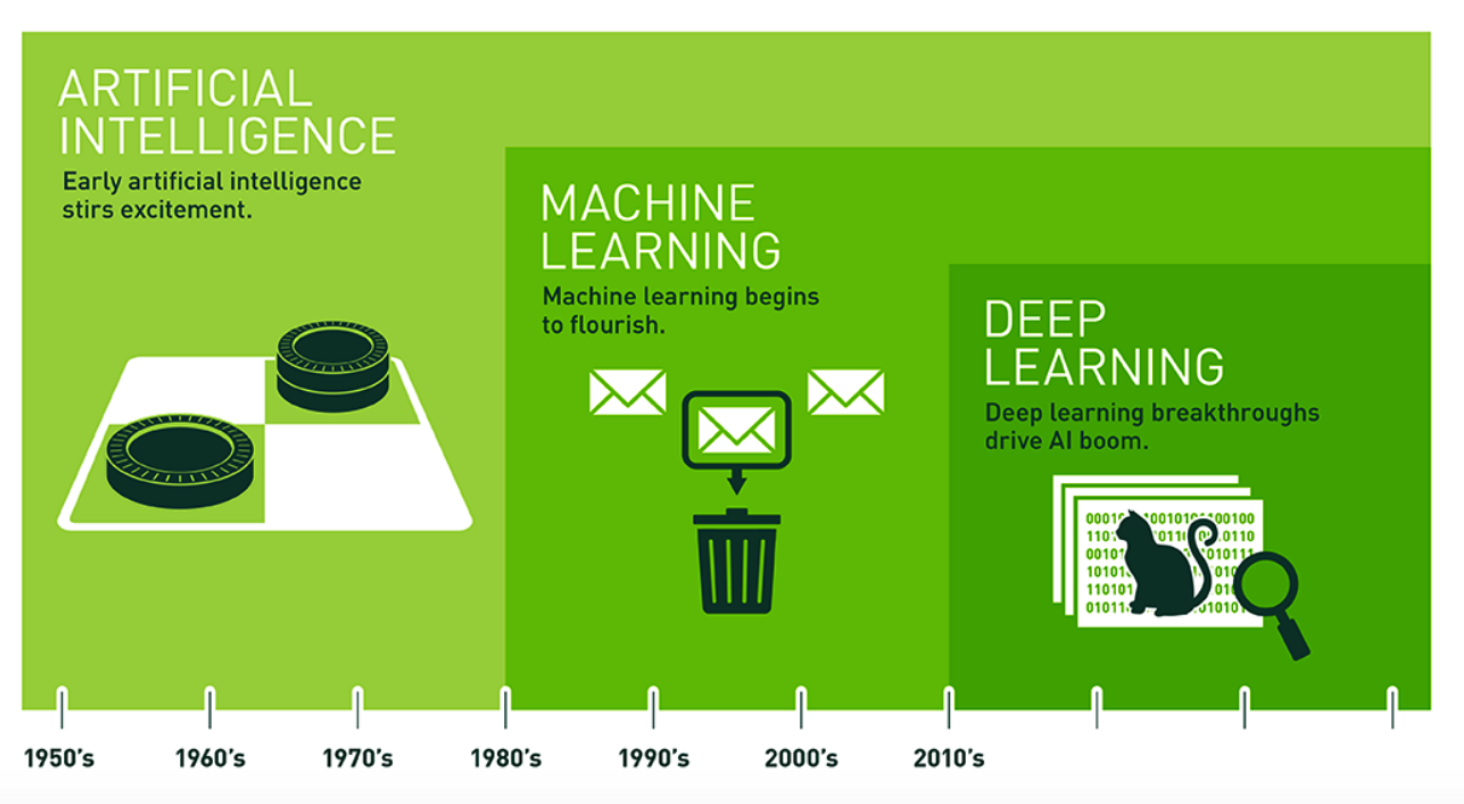
\includegraphics{./IMG/intel.png}

Machine Learning relies upon ``patterns and inference'' to ``perform a
specific task without using explicit instructions''. It is a form of
Applied AI that attempts to automatically learn from experience without
being explicitly programmed. Think of Predictive Modeling as a subset of
this which falls into two categories:

\textbf{Supervised}

Algorithms that build a model on a set of data containing both the
inputs and the desired outputs (``labels'' or known numeric values).
When you want to map input to known output labels. Build a model that,
when applied to ``new'' data, will hopefully predict the correct label.

\textbf{Unsupervised}

Algorithms that take a set of data that contains only inputs, and find
structure in the data (e.g.~clustering of data points).

This lecture is concerned primarily with Predictive Modeling. Some
examples of Predictive Modeling include:

\begin{verbatim}
Predict current CD4 cell count of an HIV-positive patient using genome sequences

Predict Success of Grant Applications

Use attributes of chemical compounds to predict likelihood of hepatic injury

How many copies of a new book will sell ?

Will a customer change Internet Service Providers ?
\end{verbatim}

A typical workflow in support of predictive modeling might look this:

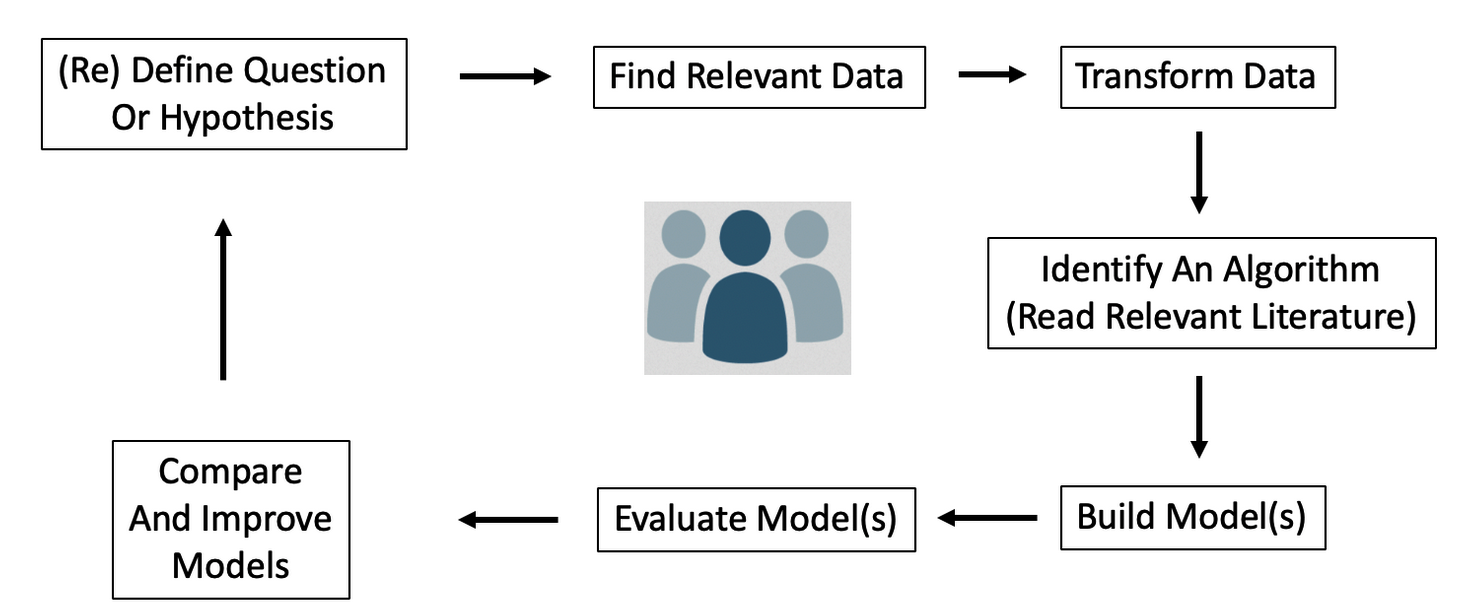
\includegraphics{./IMG/worfflow.png}

\textbf{In-Sample vs Out-Of-Sample Error}

The goal of predictive model is to generate models that can generalize
to new data. It would be good if any model we generate could provide a
good estimate of out of sample error. It's easy to generate a model on
an entire data set (in sample data) and then turn around and use that
data for prediction. But how will it perform on new data ? Haven't we
just over trained our model ?

\textbf{Performance Metrics}

For either case (regression vs classification) we need some type of
metric or measure to let us know how well a given model will work on new
or unseen data - also known as ``out of sample'' data. for
Classification problems we look at things like ``sensitivity'',
``specificity'', ``accuracy'', and ``Area Under Curve''.

For Quantitative outcomes, we look at things like Root Mean Square Error
(RMSE) or Mean Absolute Error (MAE). Here is the formula for Root Mean
Square Error (RMSE). P represents a vector of predictions and O
represents a vector of the observed (true) values.

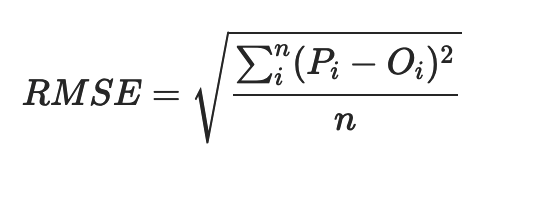
\includegraphics{./IMG/rmse.png}

\hypertarget{the-old-way---using-base-r-and-addons}{%
\subsection{The ``Old Way'' - Using Base R and
addons}\label{the-old-way---using-base-r-and-addons}}

While 'old" sounds somewhat negative, there is absolutely nothing wrong
using an established approach to model data using Base R. This involves
applying specific packages to build, for example, a logistic regression
model, a decision tree, or a support vector machine.

The job involves identifying the appropriate package(s) and then
dividing the data up in to training and testing pairs after which a
function name is called to do the work.

At a minimum, one must specify 1) the training data set and 2) a formula
which indicates what the target and predictor variables will be. Then
you look at the result

\begin{enumerate}
\def\labelenumi{\arabic{enumi})}
\tightlist
\item
  Identify appropriate packages(s) - glm, RandomForest, ranger, svm, etc
\item
  Chop up the data into a training and test pair (possibly use cross
  fold validation)
\item
  Use the right function name and pass arguments - data and prediction
  formula
\item
  Examine result using a pre-defined performance diagnostic (e.g.~RMSE,
  Accuracy, Sensitivity, AUC)
\end{enumerate}

\hypertarget{an-example}{%
\subsubsection{An Example}\label{an-example}}

Let's run through an example using the infamous \textbf{Pima Indians}
dataset to predict whether a car has an automatic transmission (0) or a
manual transmission (1). First, let's chop up the data into a training
and test pair. To get the ball rolling with a practical case, let's
consider the Pima Indians Data Frame. Read in a copy.

\begin{Shaded}
\begin{Highlighting}[]
\NormalTok{url }\OtherTok{\textless{}{-}} \StringTok{"https://raw.githubusercontent.com/steviep42/bios534\_spring\_2020/master/data/pima.csv"}
\NormalTok{pm }\OtherTok{\textless{}{-}} \FunctionTok{read.csv}\NormalTok{(url)}

\FunctionTok{head}\NormalTok{(pm)}
\end{Highlighting}
\end{Shaded}

\begin{verbatim}
##   pregnant glucose pressure triceps insulin mass pedigree age diabetes
## 1        6     148       72      35       0 33.6    0.627  50      pos
## 2        1      85       66      29       0 26.6    0.351  31      neg
## 3        8     183       64       0       0 23.3    0.672  32      pos
## 4        1      89       66      23      94 28.1    0.167  21      neg
## 5        0     137       40      35     168 43.1    2.288  33      pos
## 6        5     116       74       0       0 25.6    0.201  30      neg
\end{verbatim}

The description of the data set is as follows:

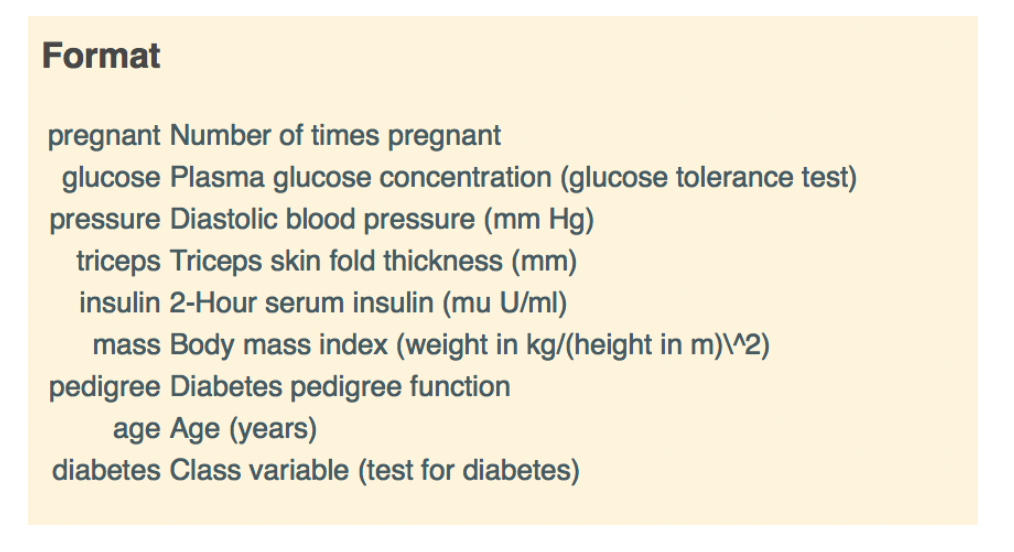
\includegraphics{./IMG/description.png}

In predictive modeling we have some important terminology:

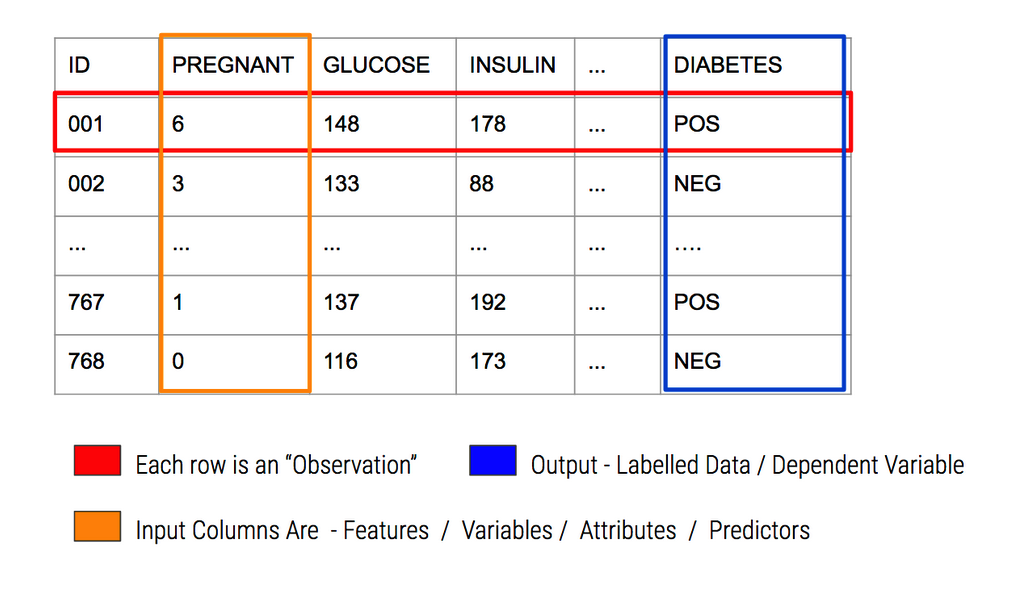
\includegraphics{./IMG/features.png}

\begin{Shaded}
\begin{Highlighting}[]
\NormalTok{corrplot}\SpecialCharTok{::}\FunctionTok{corrplot}\NormalTok{(}\FunctionTok{cor}\NormalTok{(pm[,}\SpecialCharTok{{-}}\DecValTok{9}\NormalTok{]))}
\end{Highlighting}
\end{Shaded}

\includegraphics{tidy_models_intro_files/figure-latex/unnamed-chunk-4-1.pdf}

Look at some differences between the positive vs negative cases:

\begin{Shaded}
\begin{Highlighting}[]
\NormalTok{myt }\OtherTok{\textless{}{-}} \FunctionTok{table}\NormalTok{(pm}\SpecialCharTok{$}\NormalTok{diabetes)}
\FunctionTok{barplot}\NormalTok{(myt,}
        \AttributeTok{ylim=}\FunctionTok{c}\NormalTok{(}\DecValTok{0}\NormalTok{,}\DecValTok{600}\NormalTok{),}
        \AttributeTok{main=}\StringTok{"Pima Indians {-} Count of Cases"}\NormalTok{,}
        \AttributeTok{names.arg=}\FunctionTok{names}\NormalTok{(myt),}
        \AttributeTok{ylab=}\StringTok{"Case Count"}\NormalTok{,}
        \AttributeTok{xlab=}\StringTok{"Cases"}\NormalTok{)}
\FunctionTok{grid}\NormalTok{()}
\end{Highlighting}
\end{Shaded}

\includegraphics{tidy_models_intro_files/figure-latex/unnamed-chunk-5-1.pdf}

\begin{Shaded}
\begin{Highlighting}[]
\FunctionTok{boxplot}\NormalTok{(glucose}\SpecialCharTok{\textasciitilde{}}\NormalTok{diabetes,}
        \AttributeTok{data=}\NormalTok{pm,}
        \AttributeTok{horizontal =} \ConstantTok{TRUE}\NormalTok{,}
        \AttributeTok{col=}\StringTok{"aquamarine"}\NormalTok{,}
        \AttributeTok{main=}\StringTok{"Distribution of Glucose per Group"}\NormalTok{)}
\FunctionTok{grid}\NormalTok{()}
\end{Highlighting}
\end{Shaded}

\includegraphics{tidy_models_intro_files/figure-latex/unnamed-chunk-6-1.pdf}

So let's plot Glucose vs Mass to see if any interesting hypotheses come
to mind (or not):

\begin{Shaded}
\begin{Highlighting}[]
\CommentTok{\# Split the data on the target variable which is diabetes}
\NormalTok{mysplits }\OtherTok{\textless{}{-}} \FunctionTok{split}\NormalTok{(pm,pm}\SpecialCharTok{$}\NormalTok{diabetes)}

\CommentTok{\# Create a plot window with appropriate dimensions}
\FunctionTok{plot}\NormalTok{(pm}\SpecialCharTok{$}\NormalTok{mass,pm}\SpecialCharTok{$}\NormalTok{glucose,}\AttributeTok{type=}\StringTok{"n"}\NormalTok{,}
     \AttributeTok{main=}\StringTok{"Glucose To Mass Relationship"}\NormalTok{,}
     \AttributeTok{xlab=}\StringTok{"Mass"}\NormalTok{,}
     \AttributeTok{ylab=}\StringTok{"Glucose"}\NormalTok{,}
     \AttributeTok{sub=}\StringTok{"Data from Pima Indians Data"}\NormalTok{)}

\CommentTok{\# Now put up the mass vs glucose for each group (pos and neg)}
\NormalTok{cols }\OtherTok{\textless{}{-}} \FunctionTok{c}\NormalTok{(}\StringTok{"green"}\NormalTok{,}\StringTok{"red"}\NormalTok{)}
\ControlFlowTok{for}\NormalTok{ (ii }\ControlFlowTok{in} \DecValTok{1}\SpecialCharTok{:}\FunctionTok{length}\NormalTok{(mysplits)) \{}
   \FunctionTok{points}\NormalTok{(mysplits[[ii]]}\SpecialCharTok{$}\NormalTok{mass,}
\NormalTok{          mysplits[[ii]]}\SpecialCharTok{$}\NormalTok{glucose,}
          \AttributeTok{col=}\NormalTok{cols[ii],}\AttributeTok{pch=}\DecValTok{18}\NormalTok{)  }
\NormalTok{\}}
\CommentTok{\# Draw a grid}
\FunctionTok{grid}\NormalTok{()}

\CommentTok{\# Put up a legend}
\FunctionTok{legend}\NormalTok{(}\StringTok{"topright"}\NormalTok{,}
       \AttributeTok{legend=}\FunctionTok{names}\NormalTok{(mysplits),}
       \AttributeTok{pch=}\DecValTok{18}\NormalTok{,}
       \AttributeTok{col=}\NormalTok{cols,}\AttributeTok{title=}\StringTok{"Group"}\NormalTok{)}
\end{Highlighting}
\end{Shaded}

\includegraphics{tidy_models_intro_files/figure-latex/unnamed-chunk-7-1.pdf}

\hypertarget{splitting-data-for-model-building}{%
\subsection{Splitting Data For Model
Building}\label{splitting-data-for-model-building}}

At this point we want to build a model to predict whether a given
observation will be positive for diabetes (or negative).

What we will do is create a training and testing data set using the
\textbf{sample} function. Here we will carve out rouhgly 80\% of the
data for training and 20\% for testing.

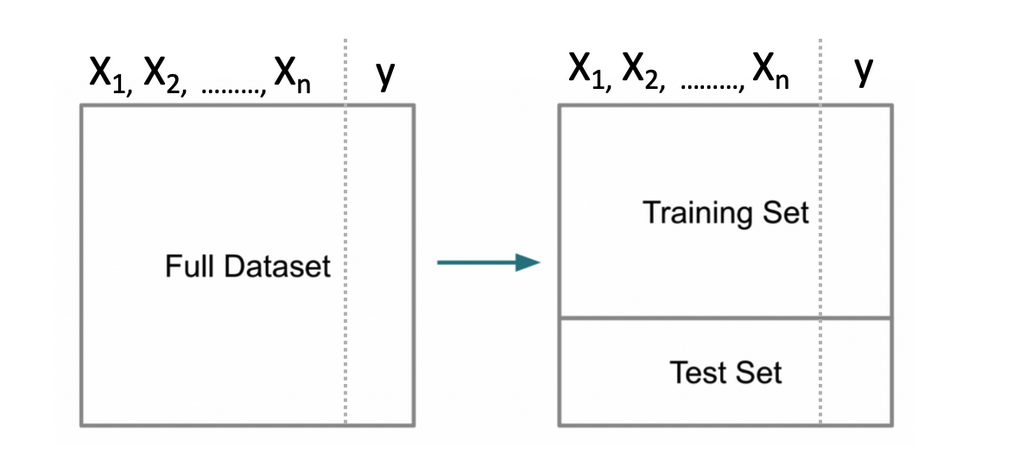
\includegraphics{./IMG/split.png}

\begin{Shaded}
\begin{Highlighting}[]
\FunctionTok{set.seed}\NormalTok{(}\DecValTok{123}\NormalTok{)  }\CommentTok{\# Makes this example reproducible}
\NormalTok{nrows }\OtherTok{\textless{}{-}} \FunctionTok{nrow}\NormalTok{(pm)}
\NormalTok{propo }\OtherTok{\textless{}{-}} \FloatTok{0.70}
\NormalTok{(idx }\OtherTok{\textless{}{-}} \FunctionTok{sample}\NormalTok{(}\DecValTok{1}\SpecialCharTok{:}\NormalTok{nrows,propo}\SpecialCharTok{*}\NormalTok{nrows))}
\end{Highlighting}
\end{Shaded}

\begin{verbatim}
##   [1] 415 463 179 526 195 118 299 229 244  14 374 665 602 603 709  91 348 649
##  [19] 355  26 519 426 751 211 590 593 555 373 143 544 490 621  23 309 135 224
##  [37] 166 217 290 581  72 588 575 141 722 153 294 277 767  41 431  90 316 223
##  [55] 528 116 606 456 598  39 159 209 758  34 516  13  69 409 308 278  89 537
##  [73] 291 424 286 671 121 110 158  64 483 477 480  67 663  85 165 648  51  74
##  [91] 178 362 236 610 330 127 212 310 243 113 619 687 151 614 160 391 155 747
## [109]   5 326 280 567 238 339 754 137 455 560 589  83 654 196 694 712 500 344
## [127] 693 459  20 764 164  52 534 177 554  84 523 392 302 597 668 650 430 428
## [145] 250 429 398 714 381 545  40 522 473 200 125 265 186 573 252 458 152  54
## [163] 538 235 289 185 413 617 735 607 205 697 564 684 701 346 664 468 509  57
## [181] 457 357 279 270 347 129 218 337 749 539 748 553 390 498 222 421 627 163
## [199] 656 704 674 225 389 117 629  55 731 557 768 134 447 104 591 210 349 401
## [217] 258 635 386 725  24 466 130 682 377 170 445 234 422 508 689  80 688 475
## [235] 696 343 323 479 450 111 317 574 287 292 226 297 681 237 628  33 746 396
## [253] 721 707  76  94 636  30 562 434 175 706 532 115 739 338  96 465 358 543
## [271] 695 661 502 580 397 404 230 148 667 556 350 425 631 423 202  81 558 503
## [289] 232 670 106 375  11 669 364 550 403 461 549  31 414 505 699 513 484  16
## [307] 197 420 678 417 412 551  12 437 609  66  50 204 579 435 741 559 384 122
## [325] 399 472 315 259 353 248 604  48 331 100 108 301  10 499 658 752 402 515
## [343] 442 653 600 395 744   8 114 261  29 306 659 679 282  73 267 738 262 733
## [361] 451 745 219 184 352 662 119 643 685 691 482  36 563 240 379 120 488 304
## [379] 432 723 449 105 281 180 547 448 241 548 167  47 191  37 174 599 303 207
## [397]  19 615 708 504 103 760 652 188 139 762 690 189 311 361 572  38 633 319
## [415] 376 334 416 546 393 371 436  21 199  87 728 497 464 520 536 517 622 367
## [433]   6 128 156 288  49 227 239 193 462 507 491 190 112 378 625 467 576 321
## [451]  59 305  61 540 525 736 750  88 132 612 251 203 246 641 460 700 366 131
## [469] 578 162 645 168 276  78 566 743  95 221 405 161 533 242 181 620 761 594
## [487] 273 187 171 313 582 136  79 638 521 400 446 427 345 646 138 719 583 686
## [505] 272 673 454 755 201 637 657 489 632   2  65 260 247 734 710 418 640 206
## [523] 124 596   7 228  45 514  25 753 470 672 268 501 263 169 711
\end{verbatim}

Now, we create the train/test pair:

\begin{Shaded}
\begin{Highlighting}[]
\NormalTok{pm}\SpecialCharTok{$}\NormalTok{diabetes }\OtherTok{\textless{}{-}} \FunctionTok{factor}\NormalTok{(pm}\SpecialCharTok{$}\NormalTok{diabetes)}
\NormalTok{pm\_training }\OtherTok{\textless{}{-}}\NormalTok{ pm[idx,]}
\NormalTok{pm\_testing  }\OtherTok{\textless{}{-}}\NormalTok{ pm[}\SpecialCharTok{{-}}\NormalTok{idx,]}

\FunctionTok{print}\NormalTok{(}\FunctionTok{paste}\NormalTok{(}\StringTok{"Training data has"}\NormalTok{,}\FunctionTok{nrow}\NormalTok{(pm\_training),}\StringTok{"rows"}\NormalTok{))}
\end{Highlighting}
\end{Shaded}

\begin{verbatim}
## [1] "Training data has 537 rows"
\end{verbatim}

\begin{Shaded}
\begin{Highlighting}[]
\FunctionTok{print}\NormalTok{(}\FunctionTok{paste}\NormalTok{(}\StringTok{"Testing data has"}\NormalTok{,}\FunctionTok{nrow}\NormalTok{(pm\_testing),}\StringTok{"rows"}\NormalTok{))}
\end{Highlighting}
\end{Shaded}

\begin{verbatim}
## [1] "Testing data has 231 rows"
\end{verbatim}

\hypertarget{a-first-model}{%
\subsection{A First Model}\label{a-first-model}}

Let's build a model using the Generalized Linear Models function. Note
that there are other types of functions we could use but most people
have at least heard of Logistic Regression so let's start with that as
it also provides us the opporunity to understand some basic ML concepts.

The \textbf{glm} function is part of Base R so you don't need to load
any additional packages to use it. We need to specify a formula, some
training data, and a ``family'' argument.

\begin{Shaded}
\begin{Highlighting}[]
\NormalTok{myglm }\OtherTok{\textless{}{-}} \FunctionTok{glm}\NormalTok{(diabetes }\SpecialCharTok{\textasciitilde{}}\NormalTok{ .,}
             \AttributeTok{data =}\NormalTok{ pm\_training,}
             \AttributeTok{family =} \StringTok{"binomial"}\NormalTok{)}

\FunctionTok{summary}\NormalTok{(myglm)}
\end{Highlighting}
\end{Shaded}

\begin{verbatim}
## 
## Call:
## glm(formula = diabetes ~ ., family = "binomial", data = pm_training)
## 
## Deviance Residuals: 
##     Min       1Q   Median       3Q      Max  
## -2.2424  -0.7256  -0.4283   0.7341   2.9311  
## 
## Coefficients:
##              Estimate Std. Error z value Pr(>|z|)    
## (Intercept) -8.405409   0.841872  -9.984  < 2e-16 ***
## pregnant     0.103471   0.037973   2.725  0.00643 ** 
## glucose      0.035730   0.004563   7.830 4.89e-15 ***
## pressure    -0.012707   0.006057  -2.098  0.03590 *  
## triceps      0.003563   0.008088   0.440  0.65959    
## insulin     -0.001710   0.001060  -1.613  0.10671    
## mass         0.088735   0.017954   4.942 7.72e-07 ***
## pedigree     0.696250   0.334761   2.080  0.03754 *  
## age          0.017015   0.011066   1.538  0.12415    
## ---
## Signif. codes:  0 '***' 0.001 '**' 0.01 '*' 0.05 '.' 0.1 ' ' 1
## 
## (Dispersion parameter for binomial family taken to be 1)
## 
##     Null deviance: 694.17  on 536  degrees of freedom
## Residual deviance: 509.76  on 528  degrees of freedom
## AIC: 527.76
## 
## Number of Fisher Scoring iterations: 5
\end{verbatim}

It's helpful to know what this object contains. Many people do not
bother to look but there is a lot of information contained therein:

\begin{Shaded}
\begin{Highlighting}[]
\FunctionTok{str}\NormalTok{(myglm)}
\end{Highlighting}
\end{Shaded}

\begin{verbatim}
## List of 30
##  $ coefficients     : Named num [1:9] -8.40541 0.10347 0.03573 -0.01271 0.00356 ...
##   ..- attr(*, "names")= chr [1:9] "(Intercept)" "pregnant" "glucose" "pressure" ...
##  $ residuals        : Named num [1:537] 2.82 -1.23 -4.17 -1.05 -1.11 ...
##   ..- attr(*, "names")= chr [1:537] "415" "463" "179" "526" ...
##  $ fitted.values    : Named num [1:537] 0.3547 0.1858 0.7605 0.0438 0.1003 ...
##   ..- attr(*, "names")= chr [1:537] "415" "463" "179" "526" ...
##  $ effects          : Named num [1:537] 4.67 -3.171 -8.547 -0.638 -1.41 ...
##   ..- attr(*, "names")= chr [1:537] "(Intercept)" "pregnant" "glucose" "pressure" ...
##  $ R                : num [1:9, 1:9] -9.11 0 0 0 0 ...
##   ..- attr(*, "dimnames")=List of 2
##   .. ..$ : chr [1:9] "(Intercept)" "pregnant" "glucose" "pressure" ...
##   .. ..$ : chr [1:9] "(Intercept)" "pregnant" "glucose" "pressure" ...
##  $ rank             : int 9
##  $ qr               :List of 5
##   ..$ qr   : num [1:537, 1:9] -9.1125 0.0427 0.0468 0.0225 0.033 ...
##   .. ..- attr(*, "dimnames")=List of 2
##   .. .. ..$ : chr [1:537] "415" "463" "179" "526" ...
##   .. .. ..$ : chr [1:9] "(Intercept)" "pregnant" "glucose" "pressure" ...
##   ..$ rank : int 9
##   ..$ qraux: num [1:9] 1.05 1.05 1.03 1 1 ...
##   ..$ pivot: int [1:9] 1 2 3 4 5 6 7 8 9
##   ..$ tol  : num 1e-11
##   ..- attr(*, "class")= chr "qr"
##  $ family           :List of 12
##   ..$ family    : chr "binomial"
##   ..$ link      : chr "logit"
##   ..$ linkfun   :function (mu)  
##   ..$ linkinv   :function (eta)  
##   ..$ variance  :function (mu)  
##   ..$ dev.resids:function (y, mu, wt)  
##   ..$ aic       :function (y, n, mu, wt, dev)  
##   ..$ mu.eta    :function (eta)  
##   ..$ initialize: language {     if (NCOL(y) == 1) { ...
##   ..$ validmu   :function (mu)  
##   ..$ valideta  :function (eta)  
##   ..$ simulate  :function (object, nsim)  
##   ..- attr(*, "class")= chr "family"
##  $ linear.predictors: Named num [1:537] -0.599 -1.478 1.155 -3.084 -2.194 ...
##   ..- attr(*, "names")= chr [1:537] "415" "463" "179" "526" ...
##  $ deviance         : num 510
##  $ aic              : num 528
##  $ null.deviance    : num 694
##  $ iter             : int 5
##  $ weights          : Named num [1:537] 0.2289 0.1513 0.1822 0.0419 0.0903 ...
##   ..- attr(*, "names")= chr [1:537] "415" "463" "179" "526" ...
##  $ prior.weights    : Named num [1:537] 1 1 1 1 1 1 1 1 1 1 ...
##   ..- attr(*, "names")= chr [1:537] "415" "463" "179" "526" ...
##  $ df.residual      : int 528
##  $ df.null          : int 536
##  $ y                : Named num [1:537] 1 0 0 0 0 0 1 0 1 1 ...
##   ..- attr(*, "names")= chr [1:537] "415" "463" "179" "526" ...
##  $ converged        : logi TRUE
##  $ boundary         : logi FALSE
##  $ model            :'data.frame':   537 obs. of  9 variables:
##   ..$ diabetes: Factor w/ 2 levels "neg","pos": 2 1 1 1 1 1 2 1 2 2 ...
##   ..$ pregnant: int [1:537] 0 8 5 3 8 5 14 4 6 1 ...
##   ..$ glucose : int [1:537] 138 74 143 87 85 78 100 197 119 189 ...
##   ..$ pressure: int [1:537] 60 70 78 60 55 48 78 70 50 60 ...
##   ..$ triceps : int [1:537] 35 40 0 18 20 0 25 39 22 23 ...
##   ..$ insulin : int [1:537] 167 49 0 0 0 0 184 744 176 846 ...
##   ..$ mass    : num [1:537] 34.6 35.3 45 21.8 24.4 33.7 36.6 36.7 27.1 30.1 ...
##   ..$ pedigree: num [1:537] 0.534 0.705 0.19 0.444 0.136 ...
##   ..$ age     : int [1:537] 21 39 47 21 42 25 46 31 33 59 ...
##   ..- attr(*, "terms")=Classes 'terms', 'formula'  language diabetes ~ pregnant + glucose + pressure + triceps + insulin + mass + pedigree +      age
##   .. .. ..- attr(*, "variables")= language list(diabetes, pregnant, glucose, pressure, triceps, insulin, mass, pedigree,      age)
##   .. .. ..- attr(*, "factors")= int [1:9, 1:8] 0 1 0 0 0 0 0 0 0 0 ...
##   .. .. .. ..- attr(*, "dimnames")=List of 2
##   .. .. .. .. ..$ : chr [1:9] "diabetes" "pregnant" "glucose" "pressure" ...
##   .. .. .. .. ..$ : chr [1:8] "pregnant" "glucose" "pressure" "triceps" ...
##   .. .. ..- attr(*, "term.labels")= chr [1:8] "pregnant" "glucose" "pressure" "triceps" ...
##   .. .. ..- attr(*, "order")= int [1:8] 1 1 1 1 1 1 1 1
##   .. .. ..- attr(*, "intercept")= int 1
##   .. .. ..- attr(*, "response")= int 1
##   .. .. ..- attr(*, ".Environment")=<environment: R_GlobalEnv> 
##   .. .. ..- attr(*, "predvars")= language list(diabetes, pregnant, glucose, pressure, triceps, insulin, mass, pedigree,      age)
##   .. .. ..- attr(*, "dataClasses")= Named chr [1:9] "factor" "numeric" "numeric" "numeric" ...
##   .. .. .. ..- attr(*, "names")= chr [1:9] "diabetes" "pregnant" "glucose" "pressure" ...
##  $ call             : language glm(formula = diabetes ~ ., family = "binomial", data = pm_training)
##  $ formula          :Class 'formula'  language diabetes ~ .
##   .. ..- attr(*, ".Environment")=<environment: R_GlobalEnv> 
##  $ terms            :Classes 'terms', 'formula'  language diabetes ~ pregnant + glucose + pressure + triceps + insulin + mass + pedigree +      age
##   .. ..- attr(*, "variables")= language list(diabetes, pregnant, glucose, pressure, triceps, insulin, mass, pedigree,      age)
##   .. ..- attr(*, "factors")= int [1:9, 1:8] 0 1 0 0 0 0 0 0 0 0 ...
##   .. .. ..- attr(*, "dimnames")=List of 2
##   .. .. .. ..$ : chr [1:9] "diabetes" "pregnant" "glucose" "pressure" ...
##   .. .. .. ..$ : chr [1:8] "pregnant" "glucose" "pressure" "triceps" ...
##   .. ..- attr(*, "term.labels")= chr [1:8] "pregnant" "glucose" "pressure" "triceps" ...
##   .. ..- attr(*, "order")= int [1:8] 1 1 1 1 1 1 1 1
##   .. ..- attr(*, "intercept")= int 1
##   .. ..- attr(*, "response")= int 1
##   .. ..- attr(*, ".Environment")=<environment: R_GlobalEnv> 
##   .. ..- attr(*, "predvars")= language list(diabetes, pregnant, glucose, pressure, triceps, insulin, mass, pedigree,      age)
##   .. ..- attr(*, "dataClasses")= Named chr [1:9] "factor" "numeric" "numeric" "numeric" ...
##   .. .. ..- attr(*, "names")= chr [1:9] "diabetes" "pregnant" "glucose" "pressure" ...
##  $ data             :'data.frame':   537 obs. of  9 variables:
##   ..$ pregnant: int [1:537] 0 8 5 3 8 5 14 4 6 1 ...
##   ..$ glucose : int [1:537] 138 74 143 87 85 78 100 197 119 189 ...
##   ..$ pressure: int [1:537] 60 70 78 60 55 48 78 70 50 60 ...
##   ..$ triceps : int [1:537] 35 40 0 18 20 0 25 39 22 23 ...
##   ..$ insulin : int [1:537] 167 49 0 0 0 0 184 744 176 846 ...
##   ..$ mass    : num [1:537] 34.6 35.3 45 21.8 24.4 33.7 36.6 36.7 27.1 30.1 ...
##   ..$ pedigree: num [1:537] 0.534 0.705 0.19 0.444 0.136 ...
##   ..$ age     : int [1:537] 21 39 47 21 42 25 46 31 33 59 ...
##   ..$ diabetes: Factor w/ 2 levels "neg","pos": 2 1 1 1 1 1 2 1 2 2 ...
##  $ offset           : NULL
##  $ control          :List of 3
##   ..$ epsilon: num 1e-08
##   ..$ maxit  : num 25
##   ..$ trace  : logi FALSE
##  $ method           : chr "glm.fit"
##  $ contrasts        : NULL
##  $ xlevels          : Named list()
##  - attr(*, "class")= chr [1:2] "glm" "lm"
\end{verbatim}

For now just observe that some of the features (e.g.~age, insulin,
triceps) do not appear to be important or significant though we'll
ignore that for now - just like a lot of professional machine learning
specialists do everyday (to their own peril).

We could do some ``feature filtering'' or ``engineering'' to first
transform or remove features to make the model diagnostics better but
that's outside of the scope of this lecture.

Let's pretend that all is well and now use this new model to predict
outcomes using the test data set. Remember that we are attempting to
predict a binary outcome - in this case whether the person is positive
for diabetes or negative.

What we get back from the prediction object are probabilities for which
we have to determine a threshold above which we would say the
observation is ``positive'' for diabetes and, below the threshold,
``negative''.

\begin{Shaded}
\begin{Highlighting}[]
\NormalTok{probs }\OtherTok{\textless{}{-}} \FunctionTok{predict}\NormalTok{(myglm,}
                 \AttributeTok{newdata =}\NormalTok{ pm\_testing,}
                 \AttributeTok{type =} \StringTok{"response"}\NormalTok{)}

\NormalTok{probs[}\DecValTok{1}\SpecialCharTok{:}\DecValTok{10}\NormalTok{]}
\end{Highlighting}
\end{Shaded}

\begin{verbatim}
##          1          3          4          9         15         17         18 
## 0.72751772 0.77340088 0.04425949 0.71110216 0.61359933 0.37579888 0.18733076 
##         22         27         28 
## 0.30034815 0.73345470 0.04357433
\end{verbatim}

With logistic regression we are dealing with a curve like the one below
which is a sigmoid function. The idea is to take our probabilities,
which range between 0 and 1, and then pick a threshold (aka ``alpha'')
over which we would classify that observation / person as being positive
for diabetes.

\begin{Shaded}
\begin{Highlighting}[]
\NormalTok{myseq }\OtherTok{\textless{}{-}} \FunctionTok{seq}\NormalTok{(}\SpecialCharTok{{-}}\DecValTok{6}\NormalTok{,}\DecValTok{6}\NormalTok{,.}\DecValTok{1}\NormalTok{)}
\NormalTok{myfunc }\OtherTok{\textless{}{-}} \ControlFlowTok{function}\NormalTok{(x) \{}\DecValTok{1}\SpecialCharTok{/}\NormalTok{(}\DecValTok{1}\SpecialCharTok{+}\FunctionTok{exp}\NormalTok{(}\SpecialCharTok{{-}}\NormalTok{x))\}}
\FunctionTok{plot}\NormalTok{(myseq,}\FunctionTok{myfunc}\NormalTok{(myseq),}
     \AttributeTok{type =} \StringTok{"l"}\NormalTok{,}
     \AttributeTok{main =} \StringTok{"Standard Logistic Sigmoid Function"}\NormalTok{,}
     \AttributeTok{ylab =} \StringTok{""}\NormalTok{)}
\FunctionTok{abline}\NormalTok{(}\AttributeTok{h=}\FloatTok{0.5}\NormalTok{,}\AttributeTok{lty=}\DecValTok{2}\NormalTok{)}
\FunctionTok{abline}\NormalTok{(}\AttributeTok{v=}\DecValTok{0}\NormalTok{,}\AttributeTok{lty=}\DecValTok{2}\NormalTok{)}
\FunctionTok{text}\NormalTok{(}\SpecialCharTok{{-}}\FloatTok{0.5}\NormalTok{,}\FloatTok{0.55}\NormalTok{,}\StringTok{"0.5"}\NormalTok{)}
\FunctionTok{grid}\NormalTok{()}
\end{Highlighting}
\end{Shaded}

\includegraphics{tidy_models_intro_files/figure-latex/unnamed-chunk-13-1.pdf}

\hypertarget{selecting-the-correct-alpha}{%
\subsubsection{Selecting The Correct
Alpha}\label{selecting-the-correct-alpha}}

The temptation is to select 0.5 as the threshold such that if a returned
probability exceeds 0.5 then we classify the associated subject as being
``positive'' for the disease. But then this assumes that the
probabilities are distributed accordingly. This is frequently not the
case though it doesn't stop people from using 0.5. Another way to view
this is as follows. This graphic shows a ``perfect'' classifier which
more or less matches the logit function above:

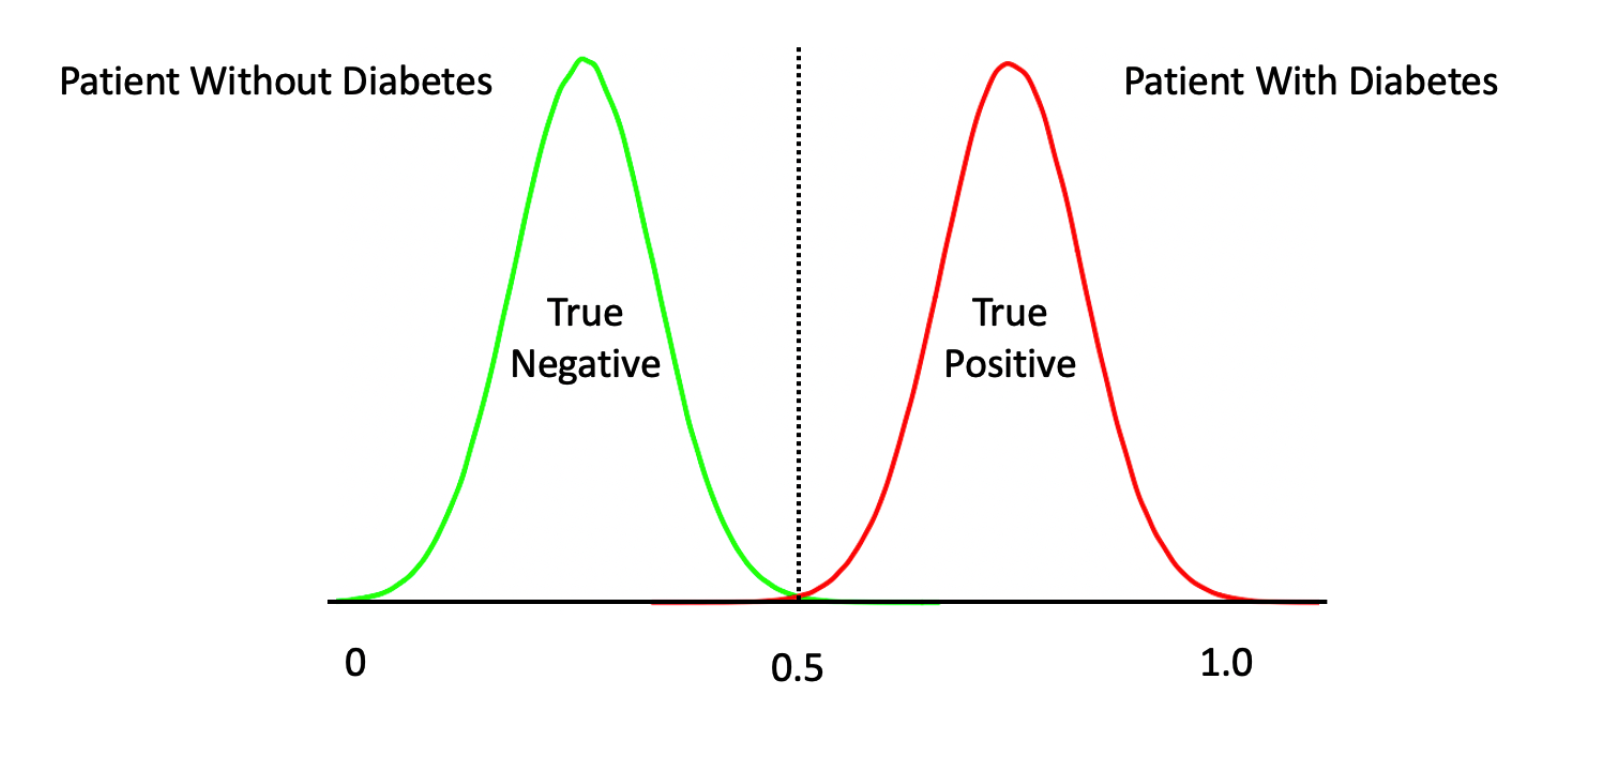
\includegraphics{./IMG/c1.png}

Note that this is a rare situation wherein there exists a clean
separation between negative and positive cases. We could more lukely
have something like this:

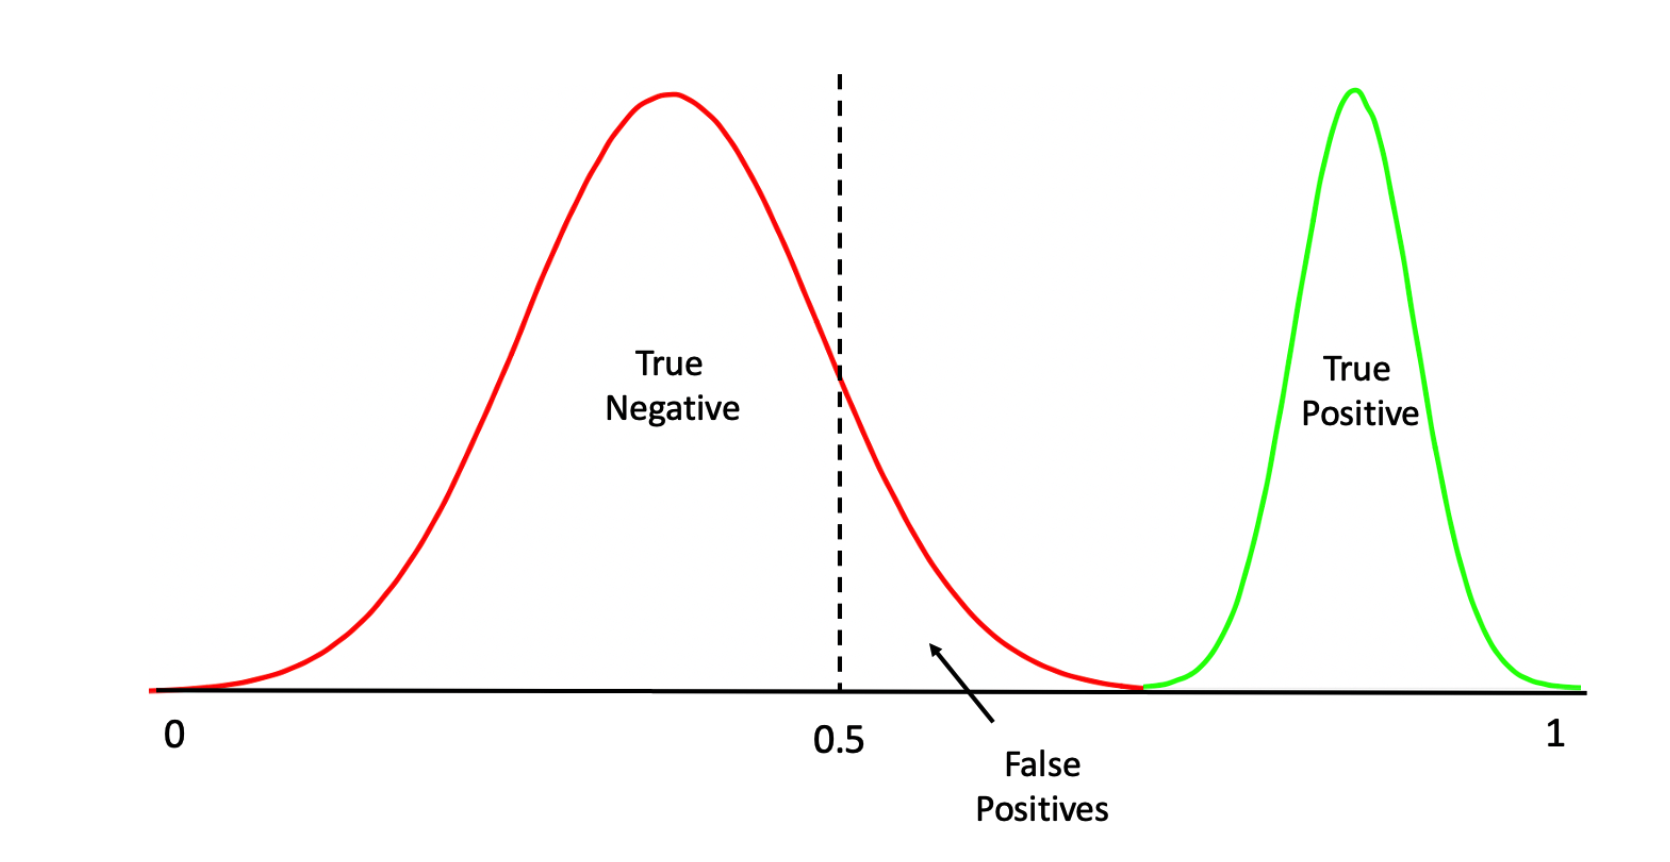
\includegraphics{./IMG/c3.png}

One thing we should do here is to look at the distribution of the
returned probabilities before making a decision about where to set the
threshold. We can see clearly that selecting 0.5 in this case would not
be appropriate.

\begin{Shaded}
\begin{Highlighting}[]
\FunctionTok{boxplot}\NormalTok{(probs, }
        \AttributeTok{main=}\StringTok{"Probabilities from our GLM Model"}\NormalTok{)}
\FunctionTok{grid}\NormalTok{()}
\end{Highlighting}
\end{Shaded}

\includegraphics{tidy_models_intro_files/figure-latex/unnamed-chunk-14-1.pdf}

The median appears to be somewhere around .25 so we could use that for
now although we are just guessing.

\begin{Shaded}
\begin{Highlighting}[]
\NormalTok{mypreds }\OtherTok{\textless{}{-}} \FunctionTok{ifelse}\NormalTok{(probs }\SpecialCharTok{\textgreater{}} \FloatTok{0.25}\NormalTok{,}\StringTok{"pos"}\NormalTok{,}\StringTok{"neg"}\NormalTok{)}
\NormalTok{mypreds }\OtherTok{\textless{}{-}} \FunctionTok{factor}\NormalTok{(mypreds, }\AttributeTok{levels =} \FunctionTok{levels}\NormalTok{(pm\_testing[[}\StringTok{"diabetes"}\NormalTok{]]))}
\NormalTok{mypreds[}\DecValTok{1}\SpecialCharTok{:}\DecValTok{10}\NormalTok{]}
\end{Highlighting}
\end{Shaded}

\begin{verbatim}
##   1   3   4   9  15  17  18  22  27  28 
## pos pos neg pos pos pos neg pos pos neg 
## Levels: neg pos
\end{verbatim}

\hypertarget{confusion-matrices}{%
\subsubsection{Confusion Matrices}\label{confusion-matrices}}

Next, we would compare our predictions against the known outcomes which
are stored in the test data frame:

\begin{Shaded}
\begin{Highlighting}[]
\CommentTok{\# How does this compare to the truth ?}
\FunctionTok{table}\NormalTok{(}\AttributeTok{predicted =}\NormalTok{ mypreds,}
      \AttributeTok{actual =}\NormalTok{ pm\_testing}\SpecialCharTok{$}\NormalTok{diabetes)}
\end{Highlighting}
\end{Shaded}

\begin{verbatim}
##          actual
## predicted neg pos
##       neg  99  16
##       pos  51  65
\end{verbatim}

What we are doing is building a ``Confusion Matrix'' which can help us
determine how effective our model is. From such a matrix table we can
compute a number of ``performance measures'', such as accuracy,
precision, sensitivity, specificity and others, to help assess the
quality of the model. In predictive modeling we are always interested in
how well any given model will perform on ``new'' data.

There are some functions that can help us compute a confusion matrix.
Because the variable we are trying to predict, (diabetes), is a two
level factor, (``neg'' or ``pos'') we'll need to turn our predictions
into a comparable factor. Right now, it's just a character string.

\begin{Shaded}
\begin{Highlighting}[]
\NormalTok{caret}\SpecialCharTok{::}\FunctionTok{confusionMatrix}\NormalTok{(mypreds,pm\_testing}\SpecialCharTok{$}\NormalTok{diabetes)}
\end{Highlighting}
\end{Shaded}

\begin{verbatim}
## Confusion Matrix and Statistics
## 
##           Reference
## Prediction neg pos
##        neg  99  16
##        pos  51  65
##                                           
##                Accuracy : 0.71            
##                  95% CI : (0.6468, 0.7676)
##     No Information Rate : 0.6494          
##     P-Value [Acc > NIR] : 0.02999         
##                                           
##                   Kappa : 0.4207          
##                                           
##  Mcnemar's Test P-Value : 3.271e-05       
##                                           
##             Sensitivity : 0.6600          
##             Specificity : 0.8025          
##          Pos Pred Value : 0.8609          
##          Neg Pred Value : 0.5603          
##              Prevalence : 0.6494          
##          Detection Rate : 0.4286          
##    Detection Prevalence : 0.4978          
##       Balanced Accuracy : 0.7312          
##                                           
##        'Positive' Class : neg             
## 
\end{verbatim}

\begin{Shaded}
\begin{Highlighting}[]
\FunctionTok{fourfoldplot}\NormalTok{(caret}\SpecialCharTok{::}\FunctionTok{confusionMatrix}\NormalTok{(mypreds,pm\_testing}\SpecialCharTok{$}\NormalTok{diabetes)}\SpecialCharTok{$}\NormalTok{table)}
\end{Highlighting}
\end{Shaded}

\includegraphics{tidy_models_intro_files/figure-latex/unnamed-chunk-17-1.pdf}

\begin{Shaded}
\begin{Highlighting}[]
\NormalTok{newpreds }\OtherTok{\textless{}{-}} \FunctionTok{ifelse}\NormalTok{(probs }\SpecialCharTok{\textgreater{}} \FloatTok{0.55}\NormalTok{,}\StringTok{"pos"}\NormalTok{,}\StringTok{"neg"}\NormalTok{)}
\NormalTok{newpreds }\OtherTok{\textless{}{-}} \FunctionTok{factor}\NormalTok{(newpreds, }\AttributeTok{levels =} \FunctionTok{levels}\NormalTok{(pm\_testing[[}\StringTok{"diabetes"}\NormalTok{]]))}
\NormalTok{newpreds[}\DecValTok{1}\SpecialCharTok{:}\DecValTok{10}\NormalTok{]}
\end{Highlighting}
\end{Shaded}

\begin{verbatim}
##   1   3   4   9  15  17  18  22  27  28 
## pos pos neg pos pos neg neg neg pos neg 
## Levels: neg pos
\end{verbatim}

\begin{Shaded}
\begin{Highlighting}[]
\FunctionTok{table}\NormalTok{(}\AttributeTok{predicted =}\NormalTok{ newpreds,}
      \AttributeTok{actual =}\NormalTok{ pm\_testing}\SpecialCharTok{$}\NormalTok{diabetes)}
\end{Highlighting}
\end{Shaded}

\begin{verbatim}
##          actual
## predicted neg pos
##       neg 141  42
##       pos   9  39
\end{verbatim}

\begin{Shaded}
\begin{Highlighting}[]
\NormalTok{caret}\SpecialCharTok{::}\FunctionTok{confusionMatrix}\NormalTok{(newpreds,pm\_testing}\SpecialCharTok{$}\NormalTok{diabetes)}
\end{Highlighting}
\end{Shaded}

\begin{verbatim}
## Confusion Matrix and Statistics
## 
##           Reference
## Prediction neg pos
##        neg 141  42
##        pos   9  39
##                                          
##                Accuracy : 0.7792         
##                  95% CI : (0.7201, 0.831)
##     No Information Rate : 0.6494         
##     P-Value [Acc > NIR] : 1.269e-05      
##                                          
##                   Kappa : 0.4651         
##                                          
##  Mcnemar's Test P-Value : 7.433e-06      
##                                          
##             Sensitivity : 0.9400         
##             Specificity : 0.4815         
##          Pos Pred Value : 0.7705         
##          Neg Pred Value : 0.8125         
##              Prevalence : 0.6494         
##          Detection Rate : 0.6104         
##    Detection Prevalence : 0.7922         
##       Balanced Accuracy : 0.7107         
##                                          
##        'Positive' Class : neg            
## 
\end{verbatim}

\begin{Shaded}
\begin{Highlighting}[]
\FunctionTok{fourfoldplot}\NormalTok{(caret}\SpecialCharTok{::}\FunctionTok{confusionMatrix}\NormalTok{(newpreds,pm\_testing}\SpecialCharTok{$}\NormalTok{diabetes)}\SpecialCharTok{$}\NormalTok{table)}
\end{Highlighting}
\end{Shaded}

\includegraphics{tidy_models_intro_files/figure-latex/unnamed-chunk-18-1.pdf}

\hypertarget{performance-measures-revisited}{%
\subsubsection{Performance Measures
Revisited}\label{performance-measures-revisited}}

This is helpful stuff although there are a number of measures to select
as a primary performance metric. Ideally, we would already know which
performance metric we would select to effectively ``judge'' the quality
of our model.

In medical tests, ``sensitivity'' and ``specificity'' are commonly used.
Some applications use ``Accuracy'' (which isn't good when there is large
group imbalance).

The problem here is that all we have done is looked at the confusion
matrix corresponding to one specific (and arbitrary) threshold value
when what we need is to look at a number of confusion matrices
corresponding to many different thresholds.

For example, we might get a better sensitivity level had we selected the
mean of the returned probabilities. This process could go on and on and
on.

\hypertarget{the-roc-curve}{%
\subsubsection{The ROC Curve}\label{the-roc-curve}}

One way to do this is to use something known as the ROC curve. Luckily,
R has functions to do this. This isn't surprising as it is a standard
tool that has been in use for decades long before the hype of AI and ML
was around. The ROC curve gives us a ``one stop shop'' for estimating a
good value of alpha.

We want to maximize the area under a given ROC curve as it winds up
being an effective way to judge the differences between one method and
another. So, if we wanted to compare the glm model against a Random
Forest model, we could use the respective AUC (Area Under Curve) metric
to help us. This isn't the only way to do this but it's reasonable for
now.

Compute the TPR and FPR for a lot of different alpha values. This is
what the ROC curve is all about:

\begin{Shaded}
\begin{Highlighting}[]
\NormalTok{pred }\OtherTok{\textless{}{-}}\NormalTok{ ROCR}\SpecialCharTok{::}\FunctionTok{prediction}\NormalTok{(}\AttributeTok{predictions =}\NormalTok{ probs,}
                         \AttributeTok{labels =}\NormalTok{ pm\_testing}\SpecialCharTok{$}\NormalTok{diabetes)}

\NormalTok{perf }\OtherTok{\textless{}{-}}\NormalTok{ ROCR}\SpecialCharTok{::}\FunctionTok{performance}\NormalTok{(pred,}
                    \StringTok{"tpr"}\NormalTok{,}
                    \StringTok{"fpr"}\NormalTok{)}

\NormalTok{myroc }\OtherTok{\textless{}{-}}\NormalTok{ ROCR}\SpecialCharTok{::}\FunctionTok{performance}\NormalTok{(pred,}\AttributeTok{measure=}\StringTok{"auc"}\NormalTok{)}

\FunctionTok{plot}\NormalTok{(perf,}\AttributeTok{colorize=}\NormalTok{T,}
        \AttributeTok{print.cutoffs.at=}\FunctionTok{seq}\NormalTok{(}\DecValTok{0}\NormalTok{,}\DecValTok{1}\NormalTok{,}\AttributeTok{by=}\FloatTok{0.1}\NormalTok{),}
     \AttributeTok{lwd=}\DecValTok{3}\NormalTok{,}\AttributeTok{las=}\DecValTok{1}\NormalTok{,}\AttributeTok{main=}\FunctionTok{paste}\NormalTok{(}\StringTok{"Cool GLM ROC Curve with"}\NormalTok{,}\FunctionTok{round}\NormalTok{(myroc}\SpecialCharTok{@}\NormalTok{y.values[[}\DecValTok{1}\NormalTok{]],}\DecValTok{3}\NormalTok{),}\StringTok{"AUC"}\NormalTok{))}
\FunctionTok{abline}\NormalTok{(}\AttributeTok{a =} \DecValTok{0}\NormalTok{, }\AttributeTok{b =} \DecValTok{1}\NormalTok{)}

\FunctionTok{grid}\NormalTok{()}
\end{Highlighting}
\end{Shaded}

\includegraphics{tidy_models_intro_files/figure-latex/unnamed-chunk-19-1.pdf}

So what value of alpha corresponds to the statedAUC of .85 ? We'll have
to dig into the performance object to get that but it looks to be
between 0.30 and 0.40. Note that this is somewhat academic since knowing
the max AUC alone helps us decide if our model is any ``good''. For
completeness we could use another R function to nail this down:

\begin{Shaded}
\begin{Highlighting}[]
\NormalTok{proc }\OtherTok{\textless{}{-}}\NormalTok{ pROC}\SpecialCharTok{::}\FunctionTok{roc}\NormalTok{(pm\_testing}\SpecialCharTok{$}\NormalTok{diabetes,probs)}
\end{Highlighting}
\end{Shaded}

\begin{verbatim}
## Setting levels: control = neg, case = pos
\end{verbatim}

\begin{verbatim}
## Setting direction: controls < cases
\end{verbatim}

\begin{Shaded}
\begin{Highlighting}[]
\FunctionTok{round}\NormalTok{(pROC}\SpecialCharTok{::}\FunctionTok{coords}\NormalTok{(proc, }\StringTok{"b"}\NormalTok{, }\AttributeTok{ret=}\StringTok{"t"}\NormalTok{, }\AttributeTok{transpose =} \ConstantTok{FALSE}\NormalTok{),}\DecValTok{2}\NormalTok{)}
\end{Highlighting}
\end{Shaded}

\begin{verbatim}
##   threshold
## 1      0.36
\end{verbatim}

We haven't accomplished very much here because we need to look at
multiple versions of the data in case we sampled a number of outliers in
the creation of our training data. Or, maybe we have excluded a large
number of outliers in the training set so they wound up in the test data
set which means that the predictive power of our model isn't as robust
as it should be.

Our next steps should involve creating multiple versions of the training
and test pairs (say 3 times), compute the optimal AUC, and then look at
how those values vary for each of those individual versions. If the AUCs
vary widely then maybe our model is over training. If it's not varying
widely, it could be that that the model has high bias.

\hypertarget{what-did-we-do}{%
\subsection{What Did We Do?}\label{what-did-we-do}}

\begin{enumerate}
\def\labelenumi{\arabic{enumi})}
\tightlist
\item
  So we chopped up some data into training and testing info
\item
  Built a model on the training data using logistic regression
\item
  Made a prediction on the test data using some arbitrary alpha value
\item
  Created a comparison between known reality and our predictions
  (confusion matrix)
\item
  We experimented with a couple of different alphas
\item
  Observed that creating a ROC curve gave us a good way to select an
  alpha
\item
  ROC curves can help us decide between one model or another.
\end{enumerate}

\hypertarget{cross-fold-validation}{%
\subsection{Cross Fold Validation}\label{cross-fold-validation}}

What if, when splitting the data into a training and testing pair, the
test set wound up containing most of the outliers in the data (assuming
there were any). This means that our trained model would probably under
perform on the test data since the model did not ``see'' most of the
outliers.

Or, consider the situation wherein the training data had most of the
outliers and the resulting model was influenced by this. So, when
applied to the testing data, the predictive results are not that great.

A way to combat this is to split the data into K number of groups aka
``folds'' - say 3. Then set up a loop that uses K-1 folds to train a
model while using the ``hold out'' fold as the test data set. This means
that each fold is used as a test set once.

It also means that each fold also gets used as part of a trained model
thus we can offset the impact of any outliers found in the data set.
Note, we are not trying to perfectly model the data, we just want to get
a realistic idea as to how it might perform on unseen data.

The method works by giving us multiple estimates of out-of-sample error,
rather than a single estimate. Let's assume K is equal to 3 so we will
partition our data into 3 individual ``folds''" which are basically
equal in size. Then we'll create a loop that does the following:

\begin{verbatim}
Combines 2 of the folds into a training data set
Builds a model on the combined 2-folds data
Applies the model to holdout fold
Computes the AUC value and stores it
\end{verbatim}

Each fold is simply a portion of the data. We'll generate a list called
``folds'' that contains 3 elements each of which are 256 index elements
corresponding to rows in pm. The way we did the sample insures that each
row shows up only in one fold.

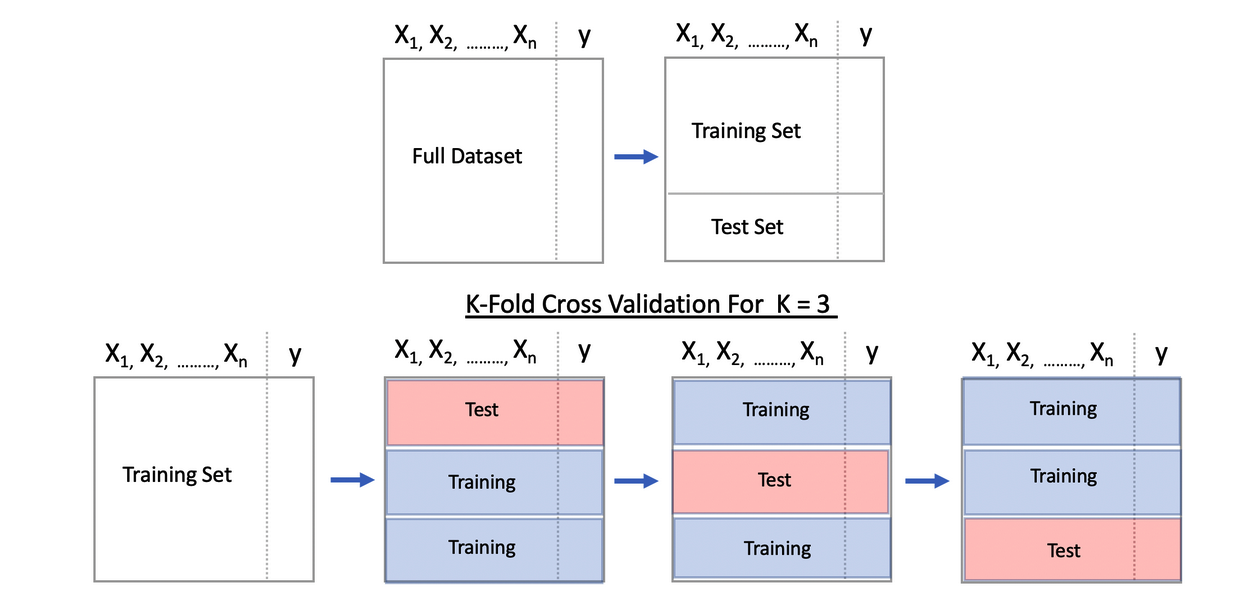
\includegraphics[width=1.2\textwidth,height=\textheight]{./IMG/crossfold.png}

We could write our own function to not only create some number of folds
but to also build a model, make predictions and store the accuracy for a
given set of folds. Remember, each fold gets to be a ``test'' data set
as part of the process.

\begin{Shaded}
\begin{Highlighting}[]
\NormalTok{cross\_fold }\OtherTok{\textless{}{-}} \ControlFlowTok{function}\NormalTok{(}\AttributeTok{numofolds =} \DecValTok{4}\NormalTok{,}\AttributeTok{df=}\NormalTok{pm) \{}
  
  \CommentTok{\# Function to Do Cross fold validation}
  
  \CommentTok{\# Split the data into K folds (numofolds)}
  
\NormalTok{  folds }\OtherTok{\textless{}{-}} \FunctionTok{split}\NormalTok{(}\FunctionTok{sample}\NormalTok{(}\DecValTok{1}\SpecialCharTok{:}\FunctionTok{nrow}\NormalTok{(df)),}\DecValTok{1}\SpecialCharTok{:}\NormalTok{numofolds) }
  
  \CommentTok{\# We setup some blank lists to stash results}
\NormalTok{  folddf    }\OtherTok{\textless{}{-}} \FunctionTok{list}\NormalTok{()  }\CommentTok{\# Contains folds}
\NormalTok{  modl      }\OtherTok{\textless{}{-}} \FunctionTok{list}\NormalTok{()  }\CommentTok{\# Hold each of the K models}
\NormalTok{  predl     }\OtherTok{\textless{}{-}} \FunctionTok{list}\NormalTok{()  }\CommentTok{\# Hold rach of the K predictions}
\NormalTok{  auc       }\OtherTok{\textless{}{-}} \FunctionTok{list}\NormalTok{()  }\CommentTok{\# Hold the auc for a given model}
  
  \CommentTok{\# Create a formula that can be used across multiple}
  \CommentTok{\# iterations through the loop. }
  
\NormalTok{  myform }\OtherTok{\textless{}{-}} \StringTok{"diabetes \textasciitilde{} ."}
  
  \ControlFlowTok{for}\NormalTok{ (ii }\ControlFlowTok{in} \DecValTok{1}\SpecialCharTok{:}\FunctionTok{length}\NormalTok{(folds)) \{}
    
    \CommentTok{\# This list holds the actual model we create for each of the }
    \CommentTok{\# 10 folds}
    
\NormalTok{    modl[[ii]] }\OtherTok{\textless{}{-}} \FunctionTok{glm}\NormalTok{(}\AttributeTok{formula =}\NormalTok{ myform, }
                      \AttributeTok{data =}\NormalTok{ df[}\SpecialCharTok{{-}}\NormalTok{folds[[ii]],],}
                      \AttributeTok{family =} \StringTok{"binomial"}\NormalTok{)}

    
    \CommentTok{\# This list will contain / hold the models build on the fold}
    
\NormalTok{    predl[[ii]]  }\OtherTok{\textless{}{-}} \FunctionTok{predict}\NormalTok{(modl[[ii]],}
                            \AttributeTok{newdata=}\NormalTok{df[folds[[ii]],],}
                            \AttributeTok{type=}\StringTok{"response"}\NormalTok{)}
   
    \CommentTok{\# This list will hold the results of the AUC per iteration}
    
\NormalTok{    pred }\OtherTok{\textless{}{-}}\NormalTok{ ROCR}\SpecialCharTok{::}\FunctionTok{prediction}\NormalTok{(predl[[ii]],}
\NormalTok{                             df[folds[[ii]],]}\SpecialCharTok{$}\NormalTok{diabetes)}
    
\NormalTok{    roc  }\OtherTok{\textless{}{-}}\NormalTok{ ROCR}\SpecialCharTok{::}\FunctionTok{performance}\NormalTok{(pred,}\AttributeTok{measure=}\StringTok{"auc"}\NormalTok{)}
\NormalTok{    auc[[ii]] }\OtherTok{\textless{}{-}}\NormalTok{ roc}\SpecialCharTok{@}\NormalTok{y.values[[}\DecValTok{1}\NormalTok{]]}
\NormalTok{  \}}
  \FunctionTok{return}\NormalTok{(}\FunctionTok{unlist}\NormalTok{(auc))}
\NormalTok{\}}
\end{Highlighting}
\end{Shaded}

Running this is now quite simple. By default, this function will loop
some number of times corresponding to the number of folds. During each
iteration it will:

\begin{verbatim}
use glm to build a model on the training folds
create a prediction object using the training fold
compute the underlying AUC associated with the prediction
store the AUC in a vector
\end{verbatim}

At the end of the function, the vector containing the computed AUCs will
be returned.

An advantage of this approach is that we can now look at a range of
accuracy values (K of them) instead of just one. This gives us a better
idea about how the model might perform on future data. Here we will look
at accuracy across 8 folds:

\begin{Shaded}
\begin{Highlighting}[]
\NormalTok{numofolds }\OtherTok{\textless{}{-}} \DecValTok{8}
\FunctionTok{boxplot}\NormalTok{(}\FunctionTok{cross\_fold}\NormalTok{(}\AttributeTok{numofolds =}\NormalTok{ numofolds),}
        \AttributeTok{main=}\FunctionTok{paste}\NormalTok{(}\StringTok{"Distribution of Accuracy for"}\NormalTok{,numofolds,}\StringTok{"folds"}\NormalTok{),}
        \AttributeTok{horizontal =} \ConstantTok{TRUE}\NormalTok{)}
\FunctionTok{grid}\NormalTok{()}
\end{Highlighting}
\end{Shaded}

\includegraphics{tidy_models_intro_files/figure-latex/unnamed-chunk-22-1.pdf}

We can even replicate this to approximate something known as repeated
cross validation:

\begin{Shaded}
\begin{Highlighting}[]
\NormalTok{numofolds }\OtherTok{\textless{}{-}} \DecValTok{8}
\NormalTok{numofrepl }\OtherTok{\textless{}{-}} \DecValTok{20}

\NormalTok{main }\OtherTok{\textless{}{-}} \FunctionTok{paste}\NormalTok{(}\StringTok{"Accuracy Across"}\NormalTok{,numofolds,}\StringTok{"folds"}\NormalTok{,}\StringTok{"}\SpecialCharTok{\textbackslash{}n}\StringTok{ and"}\NormalTok{,numofrepl,}\StringTok{"replications"}\NormalTok{)}
\NormalTok{reps }\OtherTok{\textless{}{-}} \FunctionTok{replicate}\NormalTok{(numofrepl,}\FunctionTok{cross\_fold}\NormalTok{())}

\FunctionTok{boxplot}\NormalTok{(reps,}
        \AttributeTok{main=}\NormalTok{main,}\AttributeTok{cex.axis=}\NormalTok{.}\DecValTok{8}\NormalTok{,}
        \AttributeTok{xlab=}\StringTok{"Simulation Number"}\NormalTok{,}
        \AttributeTok{ylim=}\FunctionTok{c}\NormalTok{(}\FunctionTok{min}\NormalTok{(reps)}\SpecialCharTok{{-}}\FloatTok{0.025}\NormalTok{,}\FunctionTok{max}\NormalTok{(reps)}\SpecialCharTok{+}\FloatTok{0.025}\NormalTok{),}
        \AttributeTok{ylab=}\StringTok{"Accuracy"}\NormalTok{)}
\FunctionTok{grid}\NormalTok{()}
\end{Highlighting}
\end{Shaded}

\includegraphics{tidy_models_intro_files/figure-latex/unnamed-chunk-23-1.pdf}

\hypertarget{summary}{%
\subsection{Summary}\label{summary}}

So what have we done here. Well let's recap:

\begin{enumerate}
\def\labelenumi{\arabic{enumi})}
\tightlist
\item
  Select some data and a method
\item
  Split the Data into training and testing data sets
\item
  Build a model on it and make some predictions on the test
\item
  Evaluate the model on the basis of a selected performance measure
  (e.g.~accuracy, sensitivity, AUC)
\item
  Look at plots such as ROC
\end{enumerate}

Then we might extend this by doing K-Fold cross validation at Step 2 to
get a better idea as to how the model we built might apply to the test
data. If we wanted to use another method, say random forests, we could
but that would require us to understand the calling sequence for that
method.

\hypertarget{a-different-approach}{%
\subsection{A Different Approach}\label{a-different-approach}}

We could do all of the above in a more general manner by using something
called \textbf{tidymodels}. There is also a package called
\textbf{caret} which does similar things using base R. But since the
author of \textbf{caret}, Max Kuhn, has now joined the
\textbf{tidymodels} team it seems that \textbf{caret} is in maintenance
mode only. In any case, to understand \textbf{tidymodels} one must first
understand the \textbf{tidyverse}.

The \textbf{tidyverse} represents an extension on top of the base
functions found in the default installation of R. Using \textbf{tidy}
commands is an entirely optional activity and there is no need to use
them except in pursuit of the concepts the tidyverse seeks to implement.

That sounds like circular logic but the idea is to pursue an approach
that generalizes across multiple steps in data manipulation and
modeling. Being able to easily reuse R objects (data, results, figures)
is a big deal because it simplifies the construction and comparison of
models which in turn facilitates reproducibility.

One would also like to be able to transfer knowledge acquired in using
one package to other packages in the R environment. That said, in my
view (and it's only that), having a good knowledge of base R is
important since you are likely to encounter ``legacy'' code which does
not use things like the \textbf{tidyverse} or \textbf{tidymodels}.

Some introductory courses dive straight into the \textbf{tidyverse} and
that is fine to an extent. It's just that if you enter a work
environment that has lots of older R code you will need to work to
understand it. As this presentation assumes previous experience with R
we will not be going over R basics.

\hypertarget{the-tidyverse}{%
\subsection{The tidyverse}\label{the-tidyverse}}

The \textbf{tidymodels} package comprises a number of supporting
packages and installing it is as simple as doing:

\begin{Shaded}
\begin{Highlighting}[]
\FunctionTok{install.packages}\NormalTok{(}\StringTok{"tidymodels"}\NormalTok{)}
\end{Highlighting}
\end{Shaded}

The \textbf{tidymodels} package relies on the \textbf{tidyverse} package
which provides verbs that correspond to common data manipulation
activities. The \textbf{tidyverse} package also provides the
\textbf{ggplot2} package which is a premier visualization tool. Back to
the verbs. Here are some basic examples using the \textbf{mtcars} data
frame which is frequently used in R education due its simplicity and
small size.

Let's filter the data based on values assumed by one or more columns.

\begin{Shaded}
\begin{Highlighting}[]
\FunctionTok{filter}\NormalTok{(pm, pregnant }\SpecialCharTok{\textgreater{}} \DecValTok{10} \SpecialCharTok{\&}\NormalTok{ age }\SpecialCharTok{\textless{}} \DecValTok{40}\NormalTok{)}
\end{Highlighting}
\end{Shaded}

\begin{verbatim}
##   pregnant glucose pressure triceps insulin mass pedigree age diabetes
## 1       11     138       76       0       0 33.2    0.420  35      neg
## 2       12     151       70      40     271 41.8    0.742  38      pos
## 3       14     175       62      30       0 33.6    0.212  38      pos
## 4       11      85       74       0       0 30.1    0.300  35      neg
## 5       13     104       72       0       0 31.2    0.465  38      pos
## 6       13     153       88      37     140 40.6    1.174  39      neg
\end{verbatim}

\begin{Shaded}
\begin{Highlighting}[]
\CommentTok{\# Get all rows where diabetes is "pos" and mass is \textless{} 20}
\FunctionTok{filter}\NormalTok{(pm, diabetes }\SpecialCharTok{==} \StringTok{"pos"} \SpecialCharTok{\&}\NormalTok{ mass }\SpecialCharTok{\textless{}} \DecValTok{20}\NormalTok{)}
\end{Highlighting}
\end{Shaded}

\begin{verbatim}
##   pregnant glucose pressure triceps insulin mass pedigree age diabetes
## 1        8     125       96       0       0    0    0.232  54      pos
## 2       10     115        0       0       0    0    0.261  30      pos
\end{verbatim}

We can even do aggregation using tidyverse functions. What is the
average glucose per diabetes group?

\begin{Shaded}
\begin{Highlighting}[]
\FunctionTok{summarize}\NormalTok{(}\FunctionTok{group\_by}\NormalTok{(pm,diabetes),}\AttributeTok{avg=}\FunctionTok{mean}\NormalTok{(glucose))}
\end{Highlighting}
\end{Shaded}

\begin{verbatim}
## # A tibble: 2 x 2
##   diabetes   avg
##   <fct>    <dbl>
## 1 neg       110.
## 2 pos       141.
\end{verbatim}

\hypertarget{piping}{%
\subsubsection{Piping}\label{piping}}

One of the coolest functions provided by tidyverse is the pipe operator
which allows us to feed the output of one command to the input of
another in a left-to-right fashion. This concept is now new and was
originally developed for use in the UNIX / LINUX operating system.

Base R uses composite functions in accordance of its heritage as a
mathematical / statistical language. So structures like f(g(x)) or
f(g(h(x))) are easily accommodated but prone to errors in typing due to
the need to match parentheses.

\begin{Shaded}
\begin{Highlighting}[]
\CommentTok{\# The composite function approach so Favored by mathematicians }
\NormalTok{x }\OtherTok{\textless{}{-}} \FloatTok{3.14}
\FunctionTok{log}\NormalTok{(}\FunctionTok{cos}\NormalTok{(}\FunctionTok{sin}\NormalTok{(}\FunctionTok{tan}\NormalTok{(x))),}\AttributeTok{base=}\DecValTok{10}\NormalTok{)}
\end{Highlighting}
\end{Shaded}

\begin{verbatim}
## [1] -5.508045e-07
\end{verbatim}

Using the pipe structure this would look like the following which allows
you to build the line a command at a time which makes it less error
prone. You ``read'' the command from left to right where the output of
one command becomes the input to another and so on.

\begin{Shaded}
\begin{Highlighting}[]
\NormalTok{x }\SpecialCharTok{\%\textgreater{}\%} \FunctionTok{tan}\NormalTok{() }\SpecialCharTok{\%\textgreater{}\%} \FunctionTok{sin}\NormalTok{() }\SpecialCharTok{\%\textgreater{}\%} \FunctionTok{cos}\NormalTok{() }\SpecialCharTok{\%\textgreater{}\%} \FunctionTok{log}\NormalTok{(}\AttributeTok{base=}\DecValTok{10}\NormalTok{)}
\end{Highlighting}
\end{Shaded}

\begin{verbatim}
## [1] -5.508045e-07
\end{verbatim}

\begin{Shaded}
\begin{Highlighting}[]
\CommentTok{\# or even}

\FloatTok{3.14} \SpecialCharTok{\%\textgreater{}\%} \FunctionTok{tan}\NormalTok{() }\SpecialCharTok{\%\textgreater{}\%} \FunctionTok{sin}\NormalTok{() }\SpecialCharTok{\%\textgreater{}\%} \FunctionTok{cos}\NormalTok{() }\SpecialCharTok{\%\textgreater{}\%} \FunctionTok{log}\NormalTok{(}\AttributeTok{base=}\DecValTok{10}\NormalTok{)}
\end{Highlighting}
\end{Shaded}

\begin{verbatim}
## [1] -5.508045e-07
\end{verbatim}

\begin{Shaded}
\begin{Highlighting}[]
\CommentTok{\# The pipe operator is \%\textgreater{}\%}
\NormalTok{pm  }\SpecialCharTok{\%\textgreater{}\%} \FunctionTok{filter}\NormalTok{(diabetes }\SpecialCharTok{==} \StringTok{"pos"} \SpecialCharTok{\&}\NormalTok{ mass }\SpecialCharTok{\textless{}} \DecValTok{20}\NormalTok{)}
\end{Highlighting}
\end{Shaded}

\begin{verbatim}
##   pregnant glucose pressure triceps insulin mass pedigree age diabetes
## 1        8     125       96       0       0    0    0.232  54      pos
## 2       10     115        0       0       0    0    0.261  30      pos
\end{verbatim}

We can conveniently sort data. In this case we filter out cars with MPG
greater than 15 and a weight less than 2 tons and then arrange the
result in order of highest MPG to lowest.

\begin{Shaded}
\begin{Highlighting}[]
\NormalTok{pm }\SpecialCharTok{\%\textgreater{}\%} \FunctionTok{filter}\NormalTok{(diabetes }\SpecialCharTok{==} \StringTok{"pos"} \SpecialCharTok{\&}\NormalTok{ mass }\SpecialCharTok{\textless{}} \DecValTok{25}\NormalTok{) }\SpecialCharTok{\%\textgreater{}\%} \FunctionTok{arrange}\NormalTok{(}\FunctionTok{desc}\NormalTok{(glucose))}
\end{Highlighting}
\end{Shaded}

\begin{verbatim}
##   pregnant glucose pressure triceps insulin mass pedigree age diabetes
## 1        6     194       78       0       0 23.5    0.129  59      pos
## 2        8     183       64       0       0 23.3    0.672  32      pos
## 3        1     167       74      17     144 23.4    0.447  33      pos
## 4        6     162       62       0       0 24.3    0.178  50      pos
## 5        9     156       86       0       0 24.8    0.230  53      pos
## 6        4     134       72       0       0 23.8    0.277  60      pos
## 7        8     125       96       0       0  0.0    0.232  54      pos
## 8       10     115        0       0       0  0.0    0.261  30      pos
## 9        3     107       62      13      48 22.9    0.678  23      pos
\end{verbatim}

As applied to our above grouping example we could de-couple the somewhat
verbose Base R command line:

\begin{Shaded}
\begin{Highlighting}[]
\NormalTok{pm }\SpecialCharTok{\%\textgreater{}\%} \FunctionTok{group\_by}\NormalTok{(diabetes) }\SpecialCharTok{\%\textgreater{}\%} \FunctionTok{summarize}\NormalTok{(}\AttributeTok{average\_glucose=}\FunctionTok{mean}\NormalTok{(glucose))}
\end{Highlighting}
\end{Shaded}

\begin{verbatim}
## # A tibble: 2 x 2
##   diabetes average_glucose
##   <fct>              <dbl>
## 1 neg                 110.
## 2 pos                 141.
\end{verbatim}

Note that the ``\%\textgreater\%'' operator allows us to \textbf{route}
the output of a command to the input of another command. Here is a more
simple example:

\begin{Shaded}
\begin{Highlighting}[]
\NormalTok{pm }\SpecialCharTok{\%\textgreater{}\%} \FunctionTok{filter}\NormalTok{(mass }\SpecialCharTok{\textgreater{}} \DecValTok{50}\NormalTok{)}
\end{Highlighting}
\end{Shaded}

\begin{verbatim}
##   pregnant glucose pressure triceps insulin mass pedigree age diabetes
## 1        0     162       76      56     100 53.2    0.759  25      pos
## 2        1      88       30      42      99 55.0    0.496  26      pos
## 3        0     129      110      46     130 67.1    0.319  26      pos
## 4       11     135        0       0       0 52.3    0.578  40      pos
## 5        0     165       90      33     680 52.3    0.427  23      neg
## 6        5     115       98       0       0 52.9    0.209  28      pos
## 7        0     180       78      63      14 59.4    2.420  25      pos
## 8        3     123      100      35     240 57.3    0.880  22      neg
\end{verbatim}

\begin{Shaded}
\begin{Highlighting}[]
\CommentTok{\# same as}
\FunctionTok{filter}\NormalTok{(pm, mass }\SpecialCharTok{\textgreater{}} \DecValTok{50}\NormalTok{)}
\end{Highlighting}
\end{Shaded}

\begin{verbatim}
##   pregnant glucose pressure triceps insulin mass pedigree age diabetes
## 1        0     162       76      56     100 53.2    0.759  25      pos
## 2        1      88       30      42      99 55.0    0.496  26      pos
## 3        0     129      110      46     130 67.1    0.319  26      pos
## 4       11     135        0       0       0 52.3    0.578  40      pos
## 5        0     165       90      33     680 52.3    0.427  23      neg
## 6        5     115       98       0       0 52.9    0.209  28      pos
## 7        0     180       78      63      14 59.4    2.420  25      pos
## 8        3     123      100      35     240 57.3    0.880  22      neg
\end{verbatim}

Back to our aggregation pipeline, we can ``pipe'' the result into the
ggplot function to get a visualization. ggplot requires us to provide it
tables or data frames. Actually it prefers ``tibbles'' which is a type
of data frame but that's getting off track a little bit.

\begin{Shaded}
\begin{Highlighting}[]
\NormalTok{pm }\SpecialCharTok{\%\textgreater{}\%} 
  \FunctionTok{group\_by}\NormalTok{(diabetes) }\SpecialCharTok{\%\textgreater{}\%} 
  \FunctionTok{summarize}\NormalTok{(}\AttributeTok{average\_glucose=}\FunctionTok{mean}\NormalTok{(glucose)) }\SpecialCharTok{\%\textgreater{}\%}
  \FunctionTok{ggplot}\NormalTok{(}\FunctionTok{aes}\NormalTok{(}\AttributeTok{x=}\NormalTok{diabetes,}\AttributeTok{y=}\NormalTok{average\_glucose)) }\SpecialCharTok{+} 
    \FunctionTok{geom\_bar}\NormalTok{(}\AttributeTok{stat=}\StringTok{"identity"}\NormalTok{)  }\SpecialCharTok{+} 
    \FunctionTok{ggtitle}\NormalTok{(}\StringTok{"Avg Glucose / Group"}\NormalTok{)}
\end{Highlighting}
\end{Shaded}

\includegraphics{tidy_models_intro_files/figure-latex/unnamed-chunk-32-1.pdf}

If we wanted to improve upon this we could, perhaps by making the
transmission type into a factor with more intuitive labels. Here we will
introduce another \textbf{tidyverse} function to \textbf{mutate} the
\textbf{am} variable into a factor.

\begin{Shaded}
\begin{Highlighting}[]
\NormalTok{pm }\SpecialCharTok{\%\textgreater{}\%} 
  \FunctionTok{group\_by}\NormalTok{(diabetes) }\SpecialCharTok{\%\textgreater{}\%} 
  \FunctionTok{summarize}\NormalTok{(}\AttributeTok{average\_glucose=}\FunctionTok{mean}\NormalTok{(glucose)) }\SpecialCharTok{\%\textgreater{}\%}
  \FunctionTok{ggplot}\NormalTok{(}\FunctionTok{aes}\NormalTok{(}\AttributeTok{x=}\NormalTok{diabetes,}\AttributeTok{y=}\NormalTok{average\_glucose)) }\SpecialCharTok{+} 
    \FunctionTok{geom\_bar}\NormalTok{(}\AttributeTok{stat=}\StringTok{"identity"}\NormalTok{)  }\SpecialCharTok{+} 
    \FunctionTok{theme\_light}\NormalTok{() }\SpecialCharTok{+} 
    \FunctionTok{labs}\NormalTok{(}\AttributeTok{title =} \StringTok{"Average Glucose / Group"}\NormalTok{, }
         \AttributeTok{subtitle =} \StringTok{"Data extracted from Pima Indians Data set"}\NormalTok{, }
         \AttributeTok{caption =} \StringTok{"Super Cool tidyverse example"}\NormalTok{)}
\end{Highlighting}
\end{Shaded}

\includegraphics{tidy_models_intro_files/figure-latex/unnamed-chunk-33-1.pdf}

A distinct advantage of this approach is that we did not change in
anyway the original data frame. Check it out:

\begin{Shaded}
\begin{Highlighting}[]
\FunctionTok{head}\NormalTok{(pm)}
\end{Highlighting}
\end{Shaded}

\begin{verbatim}
##   pregnant glucose pressure triceps insulin mass pedigree age diabetes
## 1        6     148       72      35       0 33.6    0.627  50      pos
## 2        1      85       66      29       0 26.6    0.351  31      neg
## 3        8     183       64       0       0 23.3    0.672  32      pos
## 4        1      89       66      23      94 28.1    0.167  21      neg
## 5        0     137       40      35     168 43.1    2.288  33      pos
## 6        5     116       74       0       0 25.6    0.201  30      neg
\end{verbatim}

The piping allows for free-form experimentation without the need for
having to save temporary and/pr incremental versions of data frames
which is frequently the case when using Base R commands. Here is another
example:

\begin{Shaded}
\begin{Highlighting}[]
\NormalTok{pm }\SpecialCharTok{\%\textgreater{}\%}
  \FunctionTok{ggplot}\NormalTok{(}\FunctionTok{aes}\NormalTok{(}\AttributeTok{x=}\NormalTok{mass,}\AttributeTok{y=}\NormalTok{glucose,}\AttributeTok{color=}\NormalTok{diabetes)) }\SpecialCharTok{+} 
  \FunctionTok{geom\_point}\NormalTok{() }\SpecialCharTok{+}
  \FunctionTok{labs}\NormalTok{(}
    \AttributeTok{title =} \StringTok{"Glucose Level vs Mass"}\NormalTok{,}
    \AttributeTok{caption =} \StringTok{"Data from the Pima Indians Data set."}\NormalTok{,}
    \AttributeTok{tag =} \StringTok{"Figure 1"}\NormalTok{,}
    \AttributeTok{x =} \StringTok{"Mass in kg(height in m)\^{}2"}\NormalTok{,}
    \AttributeTok{y =} \StringTok{"Plasma glucose concentration"}\NormalTok{,}
    \AttributeTok{colour =} \StringTok{"diabetes"}
\NormalTok{  ) }\SpecialCharTok{+} \FunctionTok{theme\_bw}\NormalTok{()}
\end{Highlighting}
\end{Shaded}

\includegraphics{tidy_models_intro_files/figure-latex/unnamed-chunk-35-1.pdf}

\hypertarget{broom---sweeping-things-up}{%
\subsubsection{Broom - sweeping things
up}\label{broom---sweeping-things-up}}

The tidyverse has a way to help clean up the results offered by Base R
packages. Consider the following:

\begin{Shaded}
\begin{Highlighting}[]
\NormalTok{fit }\OtherTok{\textless{}{-}} \FunctionTok{lm}\NormalTok{(glucose }\SpecialCharTok{\textasciitilde{}}\NormalTok{ mass }\SpecialCharTok{+}\NormalTok{ age,pm\_training)}
\end{Highlighting}
\end{Shaded}

Look at the output which is not directly in a convenient format.

\begin{Shaded}
\begin{Highlighting}[]
\NormalTok{fit}
\end{Highlighting}
\end{Shaded}

\begin{verbatim}
## 
## Call:
## lm(formula = glucose ~ mass + age, data = pm_training)
## 
## Coefficients:
## (Intercept)         mass          age  
##     68.6641       0.9534       0.6775
\end{verbatim}

\begin{Shaded}
\begin{Highlighting}[]
\FunctionTok{summary}\NormalTok{(fit)}
\end{Highlighting}
\end{Shaded}

\begin{verbatim}
## 
## Call:
## lm(formula = glucose ~ mass + age, data = pm_training)
## 
## Residuals:
##      Min       1Q   Median       3Q      Max 
## -133.625  -19.214   -1.093   18.559   83.383 
## 
## Coefficients:
##             Estimate Std. Error t value Pr(>|t|)    
## (Intercept)  68.6641     6.6155  10.379  < 2e-16 ***
## mass          0.9534     0.1663   5.732 1.66e-08 ***
## age           0.6775     0.1097   6.173 1.32e-09 ***
## ---
## Signif. codes:  0 '***' 0.001 '**' 0.01 '*' 0.05 '.' 0.1 ' ' 1
## 
## Residual standard error: 30.07 on 534 degrees of freedom
## Multiple R-squared:  0.1161, Adjusted R-squared:  0.1128 
## F-statistic: 35.07 on 2 and 534 DF,  p-value: 4.893e-15
\end{verbatim}

Access coefficients only:

\begin{Shaded}
\begin{Highlighting}[]
\NormalTok{fit}\SpecialCharTok{$}\NormalTok{coefficients}
\end{Highlighting}
\end{Shaded}

\begin{verbatim}
## (Intercept)        mass         age 
##  68.6640503   0.9534197   0.6774946
\end{verbatim}

But with a tidy approach you get things in a data frame which is
inarguably the most flexible data type in the R language. The tidy
function ``produces a tibble() where each row contains information about
an important component of the model. For regression models, this often
corresponds to regression coefficients''

\begin{Shaded}
\begin{Highlighting}[]
\FunctionTok{tidy}\NormalTok{(fit)}
\end{Highlighting}
\end{Shaded}

\begin{verbatim}
## # A tibble: 3 x 5
##   term        estimate std.error statistic  p.value
##   <chr>          <dbl>     <dbl>     <dbl>    <dbl>
## 1 (Intercept)   68.7       6.62      10.4  4.09e-23
## 2 mass           0.953     0.166      5.73 1.66e- 8
## 3 age            0.677     0.110      6.17 1.32e- 9
\end{verbatim}

The glance function ``returns a tibble with exactly one row of goodness
of fitness measures and related statistics. This is useful to check for
model misspecification and to compare many models''

\begin{Shaded}
\begin{Highlighting}[]
\FunctionTok{glance}\NormalTok{(fit)}
\end{Highlighting}
\end{Shaded}

\begin{verbatim}
## # A tibble: 1 x 12
##   r.squared adj.r.squared sigma statistic  p.value    df logLik   AIC   BIC
##       <dbl>         <dbl> <dbl>     <dbl>    <dbl> <dbl>  <dbl> <dbl> <dbl>
## 1     0.116         0.113  30.1      35.1 4.89e-15     2 -2588. 5184. 5201.
## # ... with 3 more variables: deviance <dbl>, df.residual <int>, nobs <int>
\end{verbatim}

The \textbf{augment} function ``adds columns to a dataset, containing
information such as fitted values, residuals or cluster assignments. All
columns added to a dataset have . prefix to prevent existing columns
from being overwritten.''

\begin{Shaded}
\begin{Highlighting}[]
\FunctionTok{augment}\NormalTok{(fit, pm\_training)[}\DecValTok{1}\SpecialCharTok{:}\DecValTok{10}\NormalTok{,]}
\end{Highlighting}
\end{Shaded}

\begin{verbatim}
## # A tibble: 10 x 16
##    .rownames pregnant glucose pressure triceps insulin  mass pedigree   age
##    <chr>        <int>   <int>    <int>   <int>   <int> <dbl>    <dbl> <int>
##  1 415              0     138       60      35     167  34.6    0.534    21
##  2 463              8      74       70      40      49  35.3    0.705    39
##  3 179              5     143       78       0       0  45      0.19     47
##  4 526              3      87       60      18       0  21.8    0.444    21
##  5 195              8      85       55      20       0  24.4    0.136    42
##  6 118              5      78       48       0       0  33.7    0.654    25
##  7 299             14     100       78      25     184  36.6    0.412    46
##  8 229              4     197       70      39     744  36.7    2.33     31
##  9 244              6     119       50      22     176  27.1    1.32     33
## 10 14               1     189       60      23     846  30.1    0.398    59
## # ... with 7 more variables: diabetes <fct>, .fitted <dbl>, .resid <dbl>,
## #   .hat <dbl>, .sigma <dbl>, .cooksd <dbl>, .std.resid <dbl>
\end{verbatim}

\begin{Shaded}
\begin{Highlighting}[]
\FunctionTok{augment}\NormalTok{(fit, pm\_training) }\SpecialCharTok{\%\textgreater{}\%} 
  \FunctionTok{ggplot}\NormalTok{(}\FunctionTok{aes}\NormalTok{(}\AttributeTok{x=}\NormalTok{glucose,}\AttributeTok{y=}\NormalTok{.fitted,}\AttributeTok{color=}\NormalTok{diabetes)) }\SpecialCharTok{+} 
  \FunctionTok{geom\_point}\NormalTok{() }\SpecialCharTok{+} \FunctionTok{labs}\NormalTok{(}\AttributeTok{title=}\StringTok{"Fitted vs Glucose"}\NormalTok{) }\SpecialCharTok{+} \FunctionTok{theme\_bw}\NormalTok{()}
\end{Highlighting}
\end{Shaded}

\includegraphics{tidy_models_intro_files/figure-latex/unnamed-chunk-43-1.pdf}

\hypertarget{tidymodels}{%
\subsection{Tidymodels}\label{tidymodels}}

The \textbf{tidymodels} package can be useful even if you are just
experimenting since it provides a standard and uniform approach by which
to work. In Base R, each modelling function, lm, glm, rpart, svm, will
all have arguments specific to the respective command, which contributes
to confusion when switching between models for purposes of comparison.
This is where \textbf{tidymodels} can be very helpful.

One of the benefits of the package is that it provides front ends for
the many methods available in R which includes Decision trees and
extensions there upon. An advantage of Base R when building models is
that many methods will convert the target variable to a label / nominal
feature without you asking it to. This is a convenience though the
tidyverse generally wants you do be explicit about this.

\begin{Shaded}
\begin{Highlighting}[]
\NormalTok{url }\OtherTok{\textless{}{-}} \StringTok{"https://raw.githubusercontent.com/steviep42/bios534\_spring\_2020/master/data/pima.csv"}
\NormalTok{pm }\OtherTok{\textless{}{-}} \FunctionTok{read.csv}\NormalTok{(url)}

\NormalTok{pm }\OtherTok{\textless{}{-}}\NormalTok{ pm }\SpecialCharTok{\%\textgreater{}\%} \FunctionTok{mutate}\NormalTok{(}\AttributeTok{diabetes=}\FunctionTok{factor}\NormalTok{(diabetes))}
\NormalTok{skimr}\SpecialCharTok{::}\FunctionTok{skim}\NormalTok{(pm)}
\end{Highlighting}
\end{Shaded}

\begin{longtable}[]{@{}ll@{}}
\caption{Data summary}\tabularnewline
\toprule
& \\
\midrule
\endfirsthead
\toprule
& \\
\midrule
\endhead
Name & pm \\
Number of rows & 768 \\
Number of columns & 9 \\
\_\_\_\_\_\_\_\_\_\_\_\_\_\_\_\_\_\_\_\_\_\_\_ & \\
Column type frequency: & \\
factor & 1 \\
numeric & 8 \\
\_\_\_\_\_\_\_\_\_\_\_\_\_\_\_\_\_\_\_\_\_\_\_\_ & \\
Group variables & None \\
\bottomrule
\end{longtable}

\textbf{Variable type: factor}

\begin{longtable}[]{@{}lrrlrl@{}}
\toprule
skim\_variable & n\_missing & complete\_rate & ordered & n\_unique &
top\_counts \\
\midrule
\endhead
diabetes & 0 & 1 & FALSE & 2 & neg: 500, pos: 268 \\
\bottomrule
\end{longtable}

\textbf{Variable type: numeric}

\begin{longtable}[]{@{}lrrrrrrrrrl@{}}
\toprule
skim\_variable & n\_missing & complete\_rate & mean & sd & p0 & p25 &
p50 & p75 & p100 & hist \\
\midrule
\endhead
pregnant & 0 & 1 & 3.85 & 3.37 & 0.00 & 1.00 & 3.00 & 6.00 & 17.00 &
▇▃▂▁▁ \\
glucose & 0 & 1 & 120.89 & 31.97 & 0.00 & 99.00 & 117.00 & 140.25 &
199.00 & ▁▁▇▆▂ \\
pressure & 0 & 1 & 69.11 & 19.36 & 0.00 & 62.00 & 72.00 & 80.00 & 122.00
& ▁▁▇▇▁ \\
triceps & 0 & 1 & 20.54 & 15.95 & 0.00 & 0.00 & 23.00 & 32.00 & 99.00 &
▇▇▂▁▁ \\
insulin & 0 & 1 & 79.80 & 115.24 & 0.00 & 0.00 & 30.50 & 127.25 & 846.00
& ▇▁▁▁▁ \\
mass & 0 & 1 & 31.99 & 7.88 & 0.00 & 27.30 & 32.00 & 36.60 & 67.10 &
▁▃▇▂▁ \\
pedigree & 0 & 1 & 0.47 & 0.33 & 0.08 & 0.24 & 0.37 & 0.63 & 2.42 &
▇▃▁▁▁ \\
age & 0 & 1 & 33.24 & 11.76 & 21.00 & 24.00 & 29.00 & 41.00 & 81.00 &
▇▃▁▁▁ \\
\bottomrule
\end{longtable}

\hypertarget{a-first-tidymodel}{%
\subsubsection{A First tidymodel}\label{a-first-tidymodel}}

We'll repeat our \textbf{glm} example though this time using tidymodels.
It is important to understand that the \textbf{tidymodels} package does
not attempt to replace or rewrite common and popular R packages for
model assembly.

The package provides an standard and uniform interface that ``sits on
top'' of various package functions. The advantage to the user is that
you do not necessarily need to know all of the individual arguments to a
specific command in order to use it though if you do then you can still
leverage that information.

\begin{Shaded}
\begin{Highlighting}[]
\NormalTok{pm\_tidy\_glm }\OtherTok{\textless{}{-}} \FunctionTok{logistic\_reg}\NormalTok{(}\AttributeTok{mode =} \StringTok{"classification"}\NormalTok{) }\SpecialCharTok{\%\textgreater{}\%}
  \FunctionTok{set\_engine}\NormalTok{(}\StringTok{"glm"}\NormalTok{) }
\end{Highlighting}
\end{Shaded}

\begin{Shaded}
\begin{Highlighting}[]
\NormalTok{pm\_tidy\_glm}
\end{Highlighting}
\end{Shaded}

\begin{verbatim}
## Logistic Regression Model Specification (classification)
## 
## Computational engine: glm
\end{verbatim}

Tp get more info:

\begin{Shaded}
\begin{Highlighting}[]
\NormalTok{pm\_tidy\_glm }\SpecialCharTok{\%\textgreater{}\%} \FunctionTok{translate}\NormalTok{()}
\end{Highlighting}
\end{Shaded}

\begin{verbatim}
## Logistic Regression Model Specification (classification)
## 
## Computational engine: glm 
## 
## Model fit template:
## stats::glm(formula = missing_arg(), data = missing_arg(), weights = missing_arg(), 
##     family = stats::binomial)
\end{verbatim}

\begin{Shaded}
\begin{Highlighting}[]
\NormalTok{pm\_tidy\_glm\_fit }\OtherTok{\textless{}{-}} \FunctionTok{logistic\_reg}\NormalTok{(}\AttributeTok{mode =} \StringTok{"classification"}\NormalTok{) }\SpecialCharTok{\%\textgreater{}\%}
  \FunctionTok{set\_engine}\NormalTok{(}\StringTok{"glm"}\NormalTok{) }\SpecialCharTok{\%\textgreater{}\%}
  \FunctionTok{fit}\NormalTok{(diabetes }\SpecialCharTok{\textasciitilde{}}\NormalTok{ ., }\AttributeTok{data =}\NormalTok{ pm\_training)}
\end{Highlighting}
\end{Shaded}

What do we get back?

\begin{Shaded}
\begin{Highlighting}[]
\NormalTok{pm\_tidy\_glm\_fit}
\end{Highlighting}
\end{Shaded}

\begin{verbatim}
## parsnip model object
## 
## Fit time:  4ms 
## 
## Call:  stats::glm(formula = diabetes ~ ., family = stats::binomial, 
##     data = data)
## 
## Coefficients:
## (Intercept)     pregnant      glucose     pressure      triceps      insulin  
##   -8.405409     0.103471     0.035730    -0.012707     0.003563    -0.001710  
##        mass     pedigree          age  
##    0.088735     0.696250     0.017015  
## 
## Degrees of Freedom: 536 Total (i.e. Null);  528 Residual
## Null Deviance:       694.2 
## Residual Deviance: 509.8     AIC: 527.8
\end{verbatim}

In terms of making a prediction, we can do that easily. The
\textbf{predict} function is what we call a generic function in R which
understands how to do its work based on the type of object and data that
it is being given. Remember that we built a model which returned an
object. We can pass that to the \textbf{predict} function:

\begin{Shaded}
\begin{Highlighting}[]
\FunctionTok{glance}\NormalTok{(pm\_tidy\_glm\_fit)}
\end{Highlighting}
\end{Shaded}

\begin{verbatim}
## # A tibble: 1 x 8
##   null.deviance df.null logLik   AIC   BIC deviance df.residual  nobs
##           <dbl>   <int>  <dbl> <dbl> <dbl>    <dbl>       <int> <int>
## 1          694.     536  -255.  528.  566.     510.         528   537
\end{verbatim}

\begin{Shaded}
\begin{Highlighting}[]
\CommentTok{\# Use the ranger model to make a prediction}
\NormalTok{test\_preds }\OtherTok{\textless{}{-}} \FunctionTok{predict}\NormalTok{(pm\_tidy\_glm\_fit,pm\_testing,}\AttributeTok{type=}\StringTok{"class"}\NormalTok{)}
\NormalTok{test\_preds[}\DecValTok{1}\SpecialCharTok{:}\DecValTok{10}\NormalTok{,]}
\end{Highlighting}
\end{Shaded}

\begin{verbatim}
## # A tibble: 10 x 1
##    .pred_class
##    <fct>      
##  1 pos        
##  2 pos        
##  3 neg        
##  4 pos        
##  5 pos        
##  6 neg        
##  7 neg        
##  8 neg        
##  9 pos        
## 10 neg
\end{verbatim}

Note that we also have access to probabilities which could be useful if
we needed to generate a ROC curve or wanted to take finer grained
control over thresholds.

\begin{Shaded}
\begin{Highlighting}[]
\FunctionTok{predict}\NormalTok{(pm\_tidy\_glm\_fit,}
\NormalTok{        pm\_testing,}\AttributeTok{type=}\StringTok{"prob"}\NormalTok{)[}\DecValTok{1}\SpecialCharTok{:}\DecValTok{10}\NormalTok{,]}
\end{Highlighting}
\end{Shaded}

\begin{verbatim}
## # A tibble: 10 x 2
##    .pred_neg .pred_pos
##        <dbl>     <dbl>
##  1     0.272    0.728 
##  2     0.227    0.773 
##  3     0.956    0.0443
##  4     0.289    0.711 
##  5     0.386    0.614 
##  6     0.624    0.376 
##  7     0.813    0.187 
##  8     0.700    0.300 
##  9     0.267    0.733 
## 10     0.956    0.0436
\end{verbatim}

By default we get back some predictions as to whether a subject is
positive or negative for diabetes which we could then compare to the
actual values. This would allow us to create a confusion matrix that
would then permit the computation of various performance measures such
as accuracy, sensitivity, specificity, etc.

In the tidymodels world, there are functions that will give this
information to us without the need for the confusion matrix unless we
wanted to print it.

The following shows us the predictions as part of the data frame. The
tidyverse very much likes for things to be in a data frame format -
actually something called a \textbf{tibble} which is a data frame
optimized for use with the tidyverse.

\begin{Shaded}
\begin{Highlighting}[]
\NormalTok{pm\_tidy\_glm\_fit }\SpecialCharTok{\%\textgreater{}\%}
  \FunctionTok{predict}\NormalTok{(pm\_testing) }\SpecialCharTok{\%\textgreater{}\%}
  \FunctionTok{bind\_cols}\NormalTok{(pm\_testing) }\SpecialCharTok{\%\textgreater{}\%}
  \FunctionTok{glimpse}\NormalTok{()}
\end{Highlighting}
\end{Shaded}

\begin{verbatim}
## Rows: 231
## Columns: 10
## $ .pred_class <fct> pos, pos, neg, pos, pos, neg, neg, neg, pos, neg, pos, neg~
## $ pregnant    <int> 6, 8, 1, 2, 5, 0, 7, 8, 7, 1, 3, 10, 7, 7, 9, 0, 5, 1, 0, ~
## $ glucose     <int> 148, 183, 89, 197, 166, 118, 107, 99, 147, 97, 158, 122, 1~
## $ pressure    <int> 72, 64, 66, 70, 72, 84, 74, 84, 76, 66, 76, 78, 84, 92, 11~
## $ triceps     <int> 35, 0, 23, 45, 19, 47, 0, 0, 0, 15, 36, 31, 0, 18, 24, 39,~
## $ insulin     <int> 0, 0, 94, 543, 175, 230, 0, 0, 0, 140, 245, 0, 0, 0, 240, ~
## $ mass        <dbl> 33.6, 23.3, 28.1, 30.5, 25.8, 45.8, 29.6, 35.4, 39.4, 23.2~
## $ pedigree    <dbl> 0.627, 0.672, 0.167, 0.158, 0.587, 0.551, 0.254, 0.388, 0.~
## $ age         <int> 50, 32, 21, 53, 51, 31, 31, 50, 43, 22, 28, 45, 37, 48, 54~
## $ diabetes    <fct> pos, pos, neg, pos, pos, pos, pos, neg, pos, neg, pos, neg~
\end{verbatim}

This sets the stage for evaluating the accuracy of the predictions
resulting from the model:

\begin{Shaded}
\begin{Highlighting}[]
\NormalTok{my\_metrics }\OtherTok{\textless{}{-}} \FunctionTok{metric\_set}\NormalTok{(accuracy,sensitivity,specificity, precision)}
\NormalTok{pm\_tidy\_glm\_fit }\SpecialCharTok{\%\textgreater{}\%}
  \FunctionTok{predict}\NormalTok{(pm\_testing) }\SpecialCharTok{\%\textgreater{}\%}
  \FunctionTok{bind\_cols}\NormalTok{(pm\_testing) }\SpecialCharTok{\%\textgreater{}\%}
  \FunctionTok{my\_metrics}\NormalTok{(}\AttributeTok{truth=}\NormalTok{diabetes, }\AttributeTok{estimate=}\NormalTok{.pred\_class,}\AttributeTok{event\_level =} \StringTok{"second"}\NormalTok{)}
\end{Highlighting}
\end{Shaded}

\begin{verbatim}
## # A tibble: 4 x 3
##   .metric   .estimator .estimate
##   <chr>     <chr>          <dbl>
## 1 accuracy  binary         0.792
## 2 sens      binary         0.556
## 3 spec      binary         0.92 
## 4 precision binary         0.789
\end{verbatim}

So we could derive all the metrics directly from the confusion matrix -
if we wanted to

\begin{Shaded}
\begin{Highlighting}[]
\NormalTok{pm\_tidy\_glm\_fit }\SpecialCharTok{\%\textgreater{}\%}
  \FunctionTok{predict}\NormalTok{(pm\_testing) }\SpecialCharTok{\%\textgreater{}\%}
  \FunctionTok{bind\_cols}\NormalTok{(pm\_testing) }\SpecialCharTok{\%\textgreater{}\%}
  \FunctionTok{conf\_mat}\NormalTok{(}\AttributeTok{truth=}\NormalTok{diabetes, }\AttributeTok{estimate=}\NormalTok{.pred\_class)}
\end{Highlighting}
\end{Shaded}

\begin{verbatim}
##           Truth
## Prediction neg pos
##        neg 138  36
##        pos  12  45
\end{verbatim}

But we don't need to do this as tidymodels has its own way of getting
multiple metrics all at once or a subset thereof:

\begin{Shaded}
\begin{Highlighting}[]
\NormalTok{pm\_tidy\_glm\_fit }\SpecialCharTok{\%\textgreater{}\%}
  \FunctionTok{predict}\NormalTok{(pm\_testing) }\SpecialCharTok{\%\textgreater{}\%}
  \FunctionTok{bind\_cols}\NormalTok{(pm\_testing) }\SpecialCharTok{\%\textgreater{}\%}
  \FunctionTok{conf\_mat}\NormalTok{(}\AttributeTok{truth=}\NormalTok{diabetes, }\AttributeTok{estimate=}\NormalTok{.pred\_class) }\SpecialCharTok{\%\textgreater{}\%} 
  \FunctionTok{summary}\NormalTok{(}\AttributeTok{event\_level=}\StringTok{"second"}\NormalTok{)}
\end{Highlighting}
\end{Shaded}

\begin{verbatim}
## # A tibble: 13 x 3
##    .metric              .estimator .estimate
##    <chr>                <chr>          <dbl>
##  1 accuracy             binary         0.792
##  2 kap                  binary         0.510
##  3 sens                 binary         0.556
##  4 spec                 binary         0.92 
##  5 ppv                  binary         0.789
##  6 npv                  binary         0.793
##  7 mcc                  binary         0.526
##  8 j_index              binary         0.476
##  9 bal_accuracy         binary         0.738
## 10 detection_prevalence binary         0.247
## 11 precision            binary         0.789
## 12 recall               binary         0.556
## 13 f_meas               binary         0.652
\end{verbatim}

Or you can specify just the ones you want without having to even
generate the confusion matrix

\begin{Shaded}
\begin{Highlighting}[]
\CommentTok{\# Note that sensitivity is also known as recall}
\NormalTok{my\_metrics }\OtherTok{\textless{}{-}} \FunctionTok{metric\_set}\NormalTok{(accuracy, sensitivity, specificity, precision)}
\NormalTok{pm\_tidy\_glm\_fit }\SpecialCharTok{\%\textgreater{}\%}
  \FunctionTok{predict}\NormalTok{(pm\_testing) }\SpecialCharTok{\%\textgreater{}\%}
  \FunctionTok{bind\_cols}\NormalTok{(pm\_testing) }\SpecialCharTok{\%\textgreater{}\%}
  \FunctionTok{my\_metrics}\NormalTok{(}\AttributeTok{truth=}\NormalTok{diabetes, }\AttributeTok{estimate=}\NormalTok{.pred\_class, }\AttributeTok{event\_level =} \StringTok{"second"}\NormalTok{) }
\end{Highlighting}
\end{Shaded}

\begin{verbatim}
## # A tibble: 4 x 3
##   .metric   .estimator .estimate
##   <chr>     <chr>          <dbl>
## 1 accuracy  binary         0.792
## 2 sens      binary         0.556
## 3 spec      binary         0.92 
## 4 precision binary         0.789
\end{verbatim}

And what about drawing ROC curves? The tidymodels package has that
covered. We just have to remember to get the probabilities associated
with the prediction instead of the labels.

\begin{Shaded}
\begin{Highlighting}[]
\NormalTok{pm\_tidy\_glm\_fit }\SpecialCharTok{\%\textgreater{}\%}
  \FunctionTok{predict}\NormalTok{(pm\_testing,}\AttributeTok{type=}\StringTok{"prob"}\NormalTok{) }\SpecialCharTok{\%\textgreater{}\%}      \CommentTok{\# set type="prob"}
  \FunctionTok{bind\_cols}\NormalTok{(pm\_testing) }\SpecialCharTok{\%\textgreater{}\%}
  \FunctionTok{roc\_curve}\NormalTok{(}\AttributeTok{truth=}\NormalTok{diabetes,}\AttributeTok{estimate=}\NormalTok{.pred\_pos,}\AttributeTok{event\_level=}\StringTok{"second"}\NormalTok{) }\SpecialCharTok{\%\textgreater{}\%}
  \FunctionTok{autoplot}\NormalTok{()}
\end{Highlighting}
\end{Shaded}

\includegraphics{tidy_models_intro_files/figure-latex/unnamed-chunk-58-1.pdf}
We can improve upon the default plot. First, we'll get the auc value to
use in our labels. Then we'll use this information along with various
ggplot functions.

\begin{Shaded}
\begin{Highlighting}[]
\CommentTok{\# Get the AUC}
\NormalTok{pm\_tidy\_glm\_roc\_auc }\OtherTok{\textless{}{-}}\NormalTok{ pm\_tidy\_glm\_fit }\SpecialCharTok{\%\textgreater{}\%}
  \FunctionTok{predict}\NormalTok{(pm\_testing,}\AttributeTok{type=}\StringTok{"prob"}\NormalTok{) }\SpecialCharTok{\%\textgreater{}\%}
  \FunctionTok{bind\_cols}\NormalTok{(pm\_testing) }\SpecialCharTok{\%\textgreater{}\%}
  \FunctionTok{roc\_auc}\NormalTok{(}\AttributeTok{truth=}\NormalTok{diabetes,}\AttributeTok{estimate=}\NormalTok{.pred\_pos,}\AttributeTok{event\_level=}\StringTok{"second"}\NormalTok{)}

\CommentTok{\# Put up an annotated plot}
\NormalTok{pm\_tidy\_glm\_fit }\SpecialCharTok{\%\textgreater{}\%}
  \FunctionTok{predict}\NormalTok{(pm\_testing,}\AttributeTok{type=}\StringTok{"prob"}\NormalTok{) }\SpecialCharTok{\%\textgreater{}\%}
  \FunctionTok{bind\_cols}\NormalTok{(pm\_testing) }\SpecialCharTok{\%\textgreater{}\%}
  \FunctionTok{roc\_curve}\NormalTok{(}\AttributeTok{truth=}\NormalTok{diabetes,}\AttributeTok{estimate=}\NormalTok{.pred\_pos,}\AttributeTok{event\_level=}\StringTok{"second"}\NormalTok{) }\SpecialCharTok{\%\textgreater{}\%}
  \FunctionTok{ggplot}\NormalTok{(}\FunctionTok{aes}\NormalTok{(}\AttributeTok{x=}\DecValTok{1} \SpecialCharTok{{-}}\NormalTok{ specificity, }\AttributeTok{y =}\NormalTok{ sensitivity)) }\SpecialCharTok{+} 
  \FunctionTok{geom\_path}\NormalTok{() }\SpecialCharTok{+} 
  \FunctionTok{geom\_abline}\NormalTok{(}\AttributeTok{lty=}\DecValTok{3}\NormalTok{) }\SpecialCharTok{+}
  \FunctionTok{coord\_equal}\NormalTok{() }\SpecialCharTok{+} 
  \FunctionTok{labs}\NormalTok{(}\AttributeTok{title=}\FunctionTok{paste}\NormalTok{(}\StringTok{"ROC Curve for glm with"}\NormalTok{,}\FunctionTok{round}\NormalTok{(pm\_tidy\_glm\_roc\_auc}\SpecialCharTok{$}\NormalTok{.estimate,}\DecValTok{3}\NormalTok{),}\StringTok{"AUC"}\NormalTok{)) }\SpecialCharTok{+}
  \FunctionTok{theme\_bw}\NormalTok{()}
\end{Highlighting}
\end{Shaded}

\includegraphics{tidy_models_intro_files/figure-latex/unnamed-chunk-59-1.pdf}

\hypertarget{engine-selection}{%
\subsubsection{Engine Selection}\label{engine-selection}}

Let's take a step back into the definition of the model to learn a
little more about what is happening at a basic level. So we wanted to do
logistic regression wich can be done as follows:

\begin{Shaded}
\begin{Highlighting}[]
\FunctionTok{logistic\_reg}\NormalTok{() }\SpecialCharTok{\%\textgreater{}\%} \FunctionTok{translate}\NormalTok{()}
\end{Highlighting}
\end{Shaded}

\begin{verbatim}
## Logistic Regression Model Specification (classification)
## 
## Computational engine: glm 
## 
## Model fit template:
## stats::glm(formula = missing_arg(), data = missing_arg(), weights = missing_arg(), 
##     family = stats::binomial)
\end{verbatim}

By default, the above function will select a computational engine of
``glm'' although we can choose from a number of engines which correspond
to different underlying regression methods including the following:

\begin{Shaded}
\begin{Highlighting}[]
 \FunctionTok{show\_engines}\NormalTok{(}\StringTok{"logistic\_reg"}\NormalTok{)}
\end{Highlighting}
\end{Shaded}

\begin{verbatim}
## # A tibble: 6 x 2
##   engine    mode          
##   <chr>     <chr>         
## 1 glm       classification
## 2 glmnet    classification
## 3 LiblineaR classification
## 4 spark     classification
## 5 keras     classification
## 6 stan      classification
\end{verbatim}

We can choose a different underlying method if we so desire:

\begin{Shaded}
\begin{Highlighting}[]
\FunctionTok{logistic\_reg}\NormalTok{(}\AttributeTok{mode =} \StringTok{"classification"}\NormalTok{,}\AttributeTok{penalty=}\DecValTok{1}\NormalTok{) }\SpecialCharTok{\%\textgreater{}\%} 
  \FunctionTok{set\_engine}\NormalTok{(}\StringTok{"glmnet"}\NormalTok{) }\SpecialCharTok{\%\textgreater{}\%} 
  \FunctionTok{translate}\NormalTok{()}
\end{Highlighting}
\end{Shaded}

\begin{verbatim}
## Logistic Regression Model Specification (classification)
## 
## Main Arguments:
##   penalty = 1
## 
## Computational engine: glmnet 
## 
## Model fit template:
## glmnet::glmnet(x = missing_arg(), y = missing_arg(), weights = missing_arg(), 
##     family = "binomial")
\end{verbatim}

This could be economized to:

\begin{Shaded}
\begin{Highlighting}[]
\FunctionTok{logistic\_reg}\NormalTok{(}\AttributeTok{mode =} \StringTok{"classification"}\NormalTok{,}\AttributeTok{engine=}\StringTok{"glmnet"}\NormalTok{,}\AttributeTok{penalty=}\DecValTok{1}\NormalTok{) }\SpecialCharTok{\%\textgreater{}\%} 
  \FunctionTok{translate}\NormalTok{()}
\end{Highlighting}
\end{Shaded}

\begin{verbatim}
## Logistic Regression Model Specification (classification)
## 
## Main Arguments:
##   penalty = 1
## 
## Computational engine: glmnet 
## 
## Model fit template:
## glmnet::glmnet(x = missing_arg(), y = missing_arg(), weights = missing_arg(), 
##     family = "binomial")
\end{verbatim}

\hypertarget{using-another-method}{%
\subsection{Using Another Method}\label{using-another-method}}

Jumping over to another method is easy. Let's build a random forest
using the \textbf{randomForest package}. While we provide some arguments
specific to the randomForest function we still have a lot of similarity
in our previous approach. Note, we do not have to separate the creation
of the model from the prediction phase (unless we want to).

\begin{Shaded}
\begin{Highlighting}[]
\CommentTok{\# We can get multiple metrics at once.}
\NormalTok{my\_metrics }\OtherTok{\textless{}{-}} \FunctionTok{metric\_set}\NormalTok{(accuracy, sensitivity, specificity, precision)}

\CommentTok{\# Let\textquotesingle{}s get}
\NormalTok{pm\_tidy\_preds\_rf }\OtherTok{\textless{}{-}} \FunctionTok{rand\_forest}\NormalTok{(}\AttributeTok{trees =} \DecValTok{100}\NormalTok{, }\AttributeTok{mode =} \StringTok{"classification"}\NormalTok{) }\SpecialCharTok{\%\textgreater{}\%}
  \FunctionTok{set\_engine}\NormalTok{(}\StringTok{"randomForest"}\NormalTok{) }\SpecialCharTok{\%\textgreater{}\%}
  \FunctionTok{fit}\NormalTok{(diabetes }\SpecialCharTok{\textasciitilde{}}\NormalTok{ ., }\AttributeTok{data =}\NormalTok{ pm\_training) }\SpecialCharTok{\%\textgreater{}\%}
  \FunctionTok{predict}\NormalTok{(pm\_testing) }\SpecialCharTok{\%\textgreater{}\%}
  \FunctionTok{bind\_cols}\NormalTok{(pm\_testing) }\SpecialCharTok{\%\textgreater{}\%} 
  \FunctionTok{my\_metrics}\NormalTok{(}\AttributeTok{truth=}\NormalTok{diabetes, }\AttributeTok{estimate=}\NormalTok{.pred\_class, }\AttributeTok{event\_level =} \StringTok{"second"}\NormalTok{) }

\NormalTok{pm\_tidy\_preds\_rf}
\end{Highlighting}
\end{Shaded}

\begin{verbatim}
## # A tibble: 4 x 3
##   .metric   .estimator .estimate
##   <chr>     <chr>          <dbl>
## 1 accuracy  binary         0.766
## 2 sens      binary         0.617
## 3 spec      binary         0.847
## 4 precision binary         0.685
\end{verbatim}

\hypertarget{data-management}{%
\subsection{Data Management}\label{data-management}}

So another nice thing about the tidymodels package is that it provides a
way to create and manage the training and test pair. We implemented our
own code to do this in the earlier example. While that is okay to do,
the package provides ways to do this via the \textbf{initial\_split}
function.

\hypertarget{partitioning-the-data}{%
\subsubsection{Partitioning The Data}\label{partitioning-the-data}}

\begin{Shaded}
\begin{Highlighting}[]
\FunctionTok{set.seed}\NormalTok{(}\DecValTok{123}\NormalTok{)}
\NormalTok{pm\_split }\OtherTok{\textless{}{-}} \FunctionTok{initial\_split}\NormalTok{(pm,}\AttributeTok{prop=}\FloatTok{0.7}\NormalTok{)}
\NormalTok{pm\_split}
\end{Highlighting}
\end{Shaded}

\begin{verbatim}
## <Analysis/Assess/Total>
## <537/231/768>
\end{verbatim}

This gives us a self-contained object with all the information necessary
to get the training and test data on demand. The following will access
the training data

\begin{Shaded}
\begin{Highlighting}[]
\FunctionTok{training}\NormalTok{(pm\_split)[}\DecValTok{1}\SpecialCharTok{:}\DecValTok{10}\NormalTok{,]}
\end{Highlighting}
\end{Shaded}

\begin{verbatim}
##     pregnant glucose pressure triceps insulin mass pedigree age diabetes
## 415        0     138       60      35     167 34.6    0.534  21      pos
## 463        8      74       70      40      49 35.3    0.705  39      neg
## 179        5     143       78       0       0 45.0    0.190  47      neg
## 526        3      87       60      18       0 21.8    0.444  21      neg
## 195        8      85       55      20       0 24.4    0.136  42      neg
## 118        5      78       48       0       0 33.7    0.654  25      neg
## 299       14     100       78      25     184 36.6    0.412  46      pos
## 229        4     197       70      39     744 36.7    2.329  31      neg
## 244        6     119       50      22     176 27.1    1.318  33      pos
## 14         1     189       60      23     846 30.1    0.398  59      pos
\end{verbatim}

The following will get the test data

\begin{Shaded}
\begin{Highlighting}[]
\FunctionTok{testing}\NormalTok{(pm\_split)[}\DecValTok{1}\SpecialCharTok{:}\DecValTok{10}\NormalTok{,]}
\end{Highlighting}
\end{Shaded}

\begin{verbatim}
##    pregnant glucose pressure triceps insulin mass pedigree age diabetes
## 1         6     148       72      35       0 33.6    0.627  50      pos
## 3         8     183       64       0       0 23.3    0.672  32      pos
## 4         1      89       66      23      94 28.1    0.167  21      neg
## 9         2     197       70      45     543 30.5    0.158  53      pos
## 15        5     166       72      19     175 25.8    0.587  51      pos
## 17        0     118       84      47     230 45.8    0.551  31      pos
## 18        7     107       74       0       0 29.6    0.254  31      pos
## 22        8      99       84       0       0 35.4    0.388  50      neg
## 27        7     147       76       0       0 39.4    0.257  43      pos
## 28        1      97       66      15     140 23.2    0.487  22      neg
\end{verbatim}

\hypertarget{using-the-split-data}{%
\subsubsection{Using the Split Data}\label{using-the-split-data}}

Let's repeat our glm model on the new training data. We don't expect
much difference. This is just illustrating how we can take advantage of
\textbf{tidymodels} functions to help us.

\begin{Shaded}
\begin{Highlighting}[]
\CommentTok{\# Get the Training data}
\NormalTok{pm\_training }\OtherTok{\textless{}{-}} \FunctionTok{training}\NormalTok{(pm\_split)}

\CommentTok{\# Define a model}
\NormalTok{pm\_tidy\_glm\_fit }\OtherTok{\textless{}{-}} \FunctionTok{logistic\_reg}\NormalTok{(}\AttributeTok{mode =} \StringTok{"classification"}\NormalTok{) }\SpecialCharTok{\%\textgreater{}\%}
  \FunctionTok{set\_engine}\NormalTok{(}\StringTok{"glm"}\NormalTok{) }\SpecialCharTok{\%\textgreater{}\%}
  \FunctionTok{fit}\NormalTok{(diabetes }\SpecialCharTok{\textasciitilde{}}\NormalTok{ ., }\AttributeTok{data =}\NormalTok{ pm\_training)}
\end{Highlighting}
\end{Shaded}

Now let's do some predictions using the test data

\begin{Shaded}
\begin{Highlighting}[]
\CommentTok{\# Get the Testing data}
\NormalTok{pm\_testing }\OtherTok{\textless{}{-}} \FunctionTok{testing}\NormalTok{(pm\_split)}

\CommentTok{\# Do predictions on the testing data}
\NormalTok{pm\_tidy\_glm\_fit }\SpecialCharTok{\%\textgreater{}\%}
  \FunctionTok{predict}\NormalTok{(pm\_testing) }\SpecialCharTok{\%\textgreater{}\%}
  \FunctionTok{bind\_cols}\NormalTok{(pm\_testing) }\SpecialCharTok{\%\textgreater{}\%}
  \FunctionTok{accuracy}\NormalTok{(}\AttributeTok{truth =}\NormalTok{ diabetes, }\AttributeTok{estimate =}\NormalTok{ .pred\_class)}
\end{Highlighting}
\end{Shaded}

\begin{verbatim}
## # A tibble: 1 x 3
##   .metric  .estimator .estimate
##   <chr>    <chr>          <dbl>
## 1 accuracy binary         0.792
\end{verbatim}

\hypertarget{cross-fold-validation-1}{%
\subsection{Cross Fold Validation}\label{cross-fold-validation-1}}

Just as with Base R, we can setup our data to produce a set of K folds
to help us better estimate model performance on unseen data.

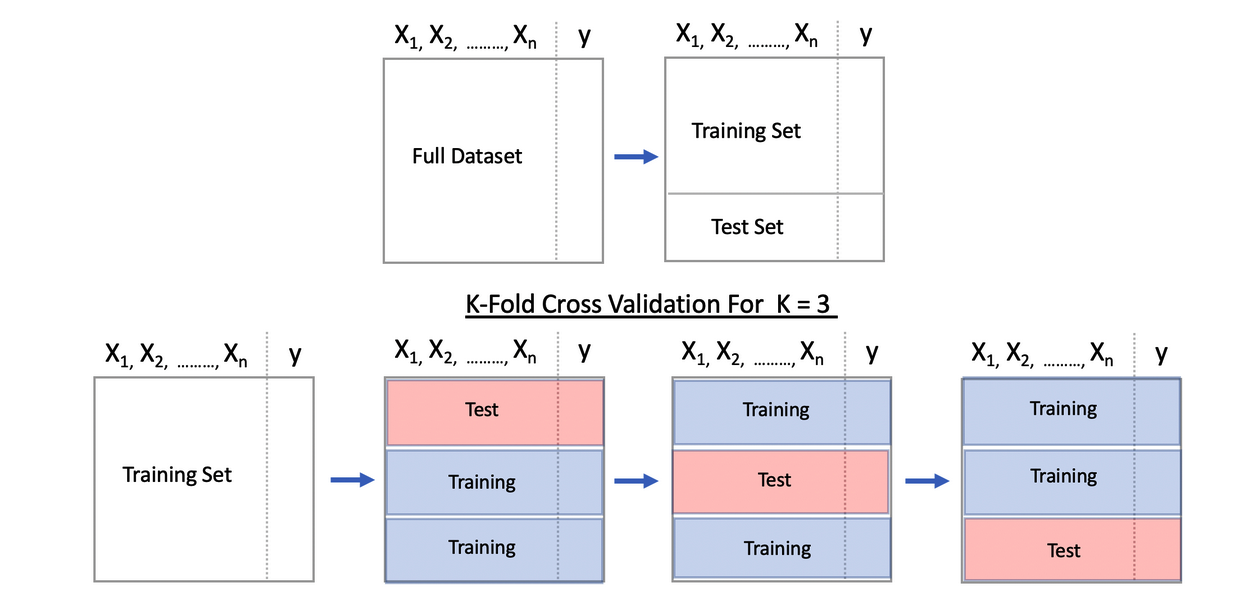
\includegraphics[width=1.2\textwidth,height=\textheight]{./IMG/crossfold.png}

We could write our own code to do this but we do not need to as
tidymodels has the \textbf{resamples} package to help us. Here we can
get 6 folds from the training data:

\begin{Shaded}
\begin{Highlighting}[]
\NormalTok{pm\_folds }\OtherTok{\textless{}{-}} \FunctionTok{vfold\_cv}\NormalTok{(pm\_training, }\AttributeTok{v =} \DecValTok{6}\NormalTok{)}
\end{Highlighting}
\end{Shaded}

So what does this structure look like?

\begin{Shaded}
\begin{Highlighting}[]
\FunctionTok{glimpse}\NormalTok{(pm\_folds)}
\end{Highlighting}
\end{Shaded}

\begin{verbatim}
## Rows: 6
## Columns: 2
## $ splits <list> [<vfold_split[447 x 90 x 537 x 9]>], [<vfold_split[447 x 90 x ~
## $ id     <chr> "Fold1", "Fold2", "Fold3", "Fold4", "Fold5", "Fold6"
\end{verbatim}

\begin{Shaded}
\begin{Highlighting}[]
\NormalTok{pm\_folds}\SpecialCharTok{$}\NormalTok{splits[[}\DecValTok{1}\NormalTok{]]}
\end{Highlighting}
\end{Shaded}

\begin{verbatim}
## <Analysis/Assess/Total>
## <447/90/537>
\end{verbatim}

\begin{Shaded}
\begin{Highlighting}[]
\NormalTok{pm\_folds}\SpecialCharTok{$}\NormalTok{splits[[}\DecValTok{1}\NormalTok{]][[}\StringTok{"data"}\NormalTok{]][}\DecValTok{1}\SpecialCharTok{:}\DecValTok{5}\NormalTok{,]}
\end{Highlighting}
\end{Shaded}

\begin{verbatim}
##     pregnant glucose pressure triceps insulin mass pedigree age diabetes
## 415        0     138       60      35     167 34.6    0.534  21      pos
## 463        8      74       70      40      49 35.3    0.705  39      neg
## 179        5     143       78       0       0 45.0    0.190  47      neg
## 526        3      87       60      18       0 21.8    0.444  21      neg
## 195        8      85       55      20       0 24.4    0.136  42      neg
\end{verbatim}

Let's repeat our exercise with fitting a model using the folds. While we
are at it, we will collect the mean accuracy and roc\_auc for this
experiment.

\begin{Shaded}
\begin{Highlighting}[]
\FunctionTok{logistic\_reg}\NormalTok{(}\AttributeTok{mode =} \StringTok{"classification"}\NormalTok{) }\SpecialCharTok{\%\textgreater{}\%}
  \FunctionTok{set\_engine}\NormalTok{(}\StringTok{"glm"}\NormalTok{) }\SpecialCharTok{\%\textgreater{}\%}
  \FunctionTok{fit\_resamples}\NormalTok{(diabetes }\SpecialCharTok{\textasciitilde{}}\NormalTok{ .,pm\_folds) }\SpecialCharTok{\%\textgreater{}\%} 
  \FunctionTok{collect\_metrics}\NormalTok{() }\SpecialCharTok{\%\textgreater{}\%} 
  \FunctionTok{select}\NormalTok{(.metric,mean,n)}
\end{Highlighting}
\end{Shaded}

\begin{verbatim}
## # A tibble: 2 x 3
##   .metric   mean     n
##   <chr>    <dbl> <int>
## 1 accuracy 0.767     6
## 2 roc_auc  0.823     6
\end{verbatim}

\hypertarget{workflows}{%
\subsection{Workflows}\label{workflows}}

Workflows allow us to consolidate a number of steps into a definition.
From the manual:

A workflow is an object that can bundle together your pre-processing,
modeling, and post-processing requests. For example, if you have a
recipe and parsnip model, these can be combined into a workflow. The
advantages are:

\begin{verbatim}
You don’t have to keep track of separate objects in your workspace.

The recipe prepping and model fitting can be executed using a single call to fit().
\end{verbatim}

Lets define a model as before

\begin{Shaded}
\begin{Highlighting}[]
\NormalTok{pm\_tidy\_glm }\OtherTok{\textless{}{-}} \FunctionTok{logistic\_reg}\NormalTok{(}\AttributeTok{mode =} \StringTok{"classification"}\NormalTok{) }\SpecialCharTok{\%\textgreater{}\%}
  \FunctionTok{set\_engine}\NormalTok{(}\StringTok{"glm"}\NormalTok{) }
\end{Highlighting}
\end{Shaded}

Next we will create a workflow to contain it. We can also add in other
things than just models but let's keep it simple for now.

\begin{Shaded}
\begin{Highlighting}[]
\NormalTok{pm\_workflow }\OtherTok{\textless{}{-}} \FunctionTok{workflow}\NormalTok{() }\SpecialCharTok{\%\textgreater{}\%}
  \FunctionTok{add\_formula}\NormalTok{(diabetes}\SpecialCharTok{\textasciitilde{}}\NormalTok{.) }\SpecialCharTok{\%\textgreater{}\%} 
  \FunctionTok{add\_model}\NormalTok{(pm\_tidy\_glm)}
\end{Highlighting}
\end{Shaded}

Check it out:

\begin{Shaded}
\begin{Highlighting}[]
\NormalTok{pm\_workflow}
\end{Highlighting}
\end{Shaded}

\begin{verbatim}
## == Workflow ====================================================================
## Preprocessor: Formula
## Model: logistic_reg()
## 
## -- Preprocessor ----------------------------------------------------------------
## diabetes ~ .
## 
## -- Model -----------------------------------------------------------------------
## Logistic Regression Model Specification (classification)
## 
## Computational engine: glm
\end{verbatim}

Before we do anything with it, I wanted to point out that you could
update specific components of an existing wrokflow. This is helpful if
our workflow defintition has lots of individual components to it. In
this case we do not have that many but this is a good time to point out
the advantage of being able to update a workflow.

\begin{Shaded}
\begin{Highlighting}[]
\FunctionTok{update\_formula}\NormalTok{(pm\_workflow,diabetes}\SpecialCharTok{\textasciitilde{}}\NormalTok{mass)}
\end{Highlighting}
\end{Shaded}

\begin{verbatim}
## == Workflow ====================================================================
## Preprocessor: Formula
## Model: logistic_reg()
## 
## -- Preprocessor ----------------------------------------------------------------
## diabetes ~ mass
## 
## -- Model -----------------------------------------------------------------------
## Logistic Regression Model Specification (classification)
## 
## Computational engine: glm
\end{verbatim}

So we can execute the workflow by ``fitting'' it.

\begin{Shaded}
\begin{Highlighting}[]
\NormalTok{pm\_workflow\_fit }\OtherTok{\textless{}{-}} \FunctionTok{fit}\NormalTok{(pm\_workflow,}\AttributeTok{data=}\NormalTok{pm\_training)}
\end{Highlighting}
\end{Shaded}

And then predictions can be made:

\begin{Shaded}
\begin{Highlighting}[]
\FunctionTok{predict}\NormalTok{(pm\_workflow\_fit,pm\_testing) }\SpecialCharTok{\%\textgreater{}\%}
  \FunctionTok{bind\_cols}\NormalTok{(}\AttributeTok{new\_data=}\NormalTok{pm\_testing) }\SpecialCharTok{\%\textgreater{}\%}
  \FunctionTok{my\_metrics}\NormalTok{(}\AttributeTok{truth=}\NormalTok{diabetes, }\AttributeTok{estimate=}\NormalTok{.pred\_class,}\AttributeTok{event\_level=}\StringTok{"second"}\NormalTok{) }
\end{Highlighting}
\end{Shaded}

\begin{verbatim}
## # A tibble: 4 x 3
##   .metric   .estimator .estimate
##   <chr>     <chr>          <dbl>
## 1 accuracy  binary         0.792
## 2 sens      binary         0.556
## 3 spec      binary         0.92 
## 4 precision binary         0.789
\end{verbatim}

This could be done in one go if desired. Those facile with tidy commands
might prefer this although you are encouraged to keep things simple if
you wish. You can break up the pipeline into segments wherein you save
information along the way.

\begin{Shaded}
\begin{Highlighting}[]
\FunctionTok{workflow}\NormalTok{() }\SpecialCharTok{\%\textgreater{}\%}
  \FunctionTok{add\_formula}\NormalTok{(diabetes}\SpecialCharTok{\textasciitilde{}}\NormalTok{.) }\SpecialCharTok{\%\textgreater{}\%} 
  \FunctionTok{add\_model}\NormalTok{(pm\_tidy\_glm) }\SpecialCharTok{\%\textgreater{}\%} 
  \FunctionTok{fit}\NormalTok{(}\AttributeTok{data=}\NormalTok{pm\_training) }\SpecialCharTok{\%\textgreater{}\%}
  \FunctionTok{predict}\NormalTok{(}\AttributeTok{new\_data=}\NormalTok{pm\_testing) }\SpecialCharTok{\%\textgreater{}\%}
  \FunctionTok{bind\_cols}\NormalTok{(pm\_testing) }\SpecialCharTok{\%\textgreater{}\%}
  \FunctionTok{my\_metrics}\NormalTok{(}\AttributeTok{truth=}\NormalTok{diabetes, }\AttributeTok{estimate=}\NormalTok{.pred\_class,}\AttributeTok{event\_level=}\StringTok{"second"}\NormalTok{) }
\end{Highlighting}
\end{Shaded}

\begin{verbatim}
## # A tibble: 4 x 3
##   .metric   .estimator .estimate
##   <chr>     <chr>          <dbl>
## 1 accuracy  binary         0.792
## 2 sens      binary         0.556
## 3 spec      binary         0.92 
## 4 precision binary         0.789
\end{verbatim}

What else can we do with workflows ? What about cross validation ? Yes!
Let's define everything from scratch which should serve as a review

\begin{Shaded}
\begin{Highlighting}[]
\CommentTok{\# Define the model}
\NormalTok{pm\_tidy\_glm }\OtherTok{\textless{}{-}} \FunctionTok{logistic\_reg}\NormalTok{(}\AttributeTok{mode =} \StringTok{"classification"}\NormalTok{) }\SpecialCharTok{\%\textgreater{}\%}
  \FunctionTok{set\_engine}\NormalTok{(}\StringTok{"glm"}\NormalTok{) }

\CommentTok{\# Define the workflow}
\NormalTok{pm\_workflow }\OtherTok{\textless{}{-}} \FunctionTok{workflow}\NormalTok{() }\SpecialCharTok{\%\textgreater{}\%}
  \FunctionTok{add\_formula}\NormalTok{(diabetes}\SpecialCharTok{\textasciitilde{}}\NormalTok{.) }\SpecialCharTok{\%\textgreater{}\%} 
  \FunctionTok{add\_model}\NormalTok{(pm\_tidy\_glm)}
\end{Highlighting}
\end{Shaded}

So if we wanted to train the model on a set of folds how would we do
that? Where would we specify it in the workflow? First, we can create
the folds using the following:

\begin{Shaded}
\begin{Highlighting}[]
\CommentTok{\# Create 6 folds}
\NormalTok{pm\_folds }\OtherTok{\textless{}{-}} \FunctionTok{vfold\_cv}\NormalTok{(}\FunctionTok{training}\NormalTok{(pm\_split), }\AttributeTok{v =} \DecValTok{6}\NormalTok{)}
\FunctionTok{glimpse}\NormalTok{(pm\_folds)}
\end{Highlighting}
\end{Shaded}

\begin{verbatim}
## Rows: 6
## Columns: 2
## $ splits <list> [<vfold_split[447 x 90 x 537 x 9]>], [<vfold_split[447 x 90 x ~
## $ id     <chr> "Fold1", "Fold2", "Fold3", "Fold4", "Fold5", "Fold6"
\end{verbatim}

Back to the question of how to get these folds to be used in the
training / fitting process?

\begin{Shaded}
\begin{Highlighting}[]
\CommentTok{\# We can use the fit\_resamples function to do a fit that uses the folds}
\NormalTok{log\_fit }\OtherTok{\textless{}{-}} \FunctionTok{fit\_resamples}\NormalTok{(pm\_workflow, }
\NormalTok{                         pm\_folds, }
                         \AttributeTok{metrics =}\NormalTok{ my\_metrics,}
                         \AttributeTok{control =} \FunctionTok{control\_resamples}\NormalTok{(}\AttributeTok{event\_level =} \StringTok{"second"}\NormalTok{)) }\SpecialCharTok{\%\textgreater{}\%}
  \FunctionTok{collect\_metrics}\NormalTok{()}
\end{Highlighting}
\end{Shaded}

What do we get for our trouble ?

\begin{Shaded}
\begin{Highlighting}[]
\NormalTok{log\_fit}
\end{Highlighting}
\end{Shaded}

\begin{verbatim}
## # A tibble: 4 x 6
##   .metric   .estimator  mean     n std_err .config             
##   <chr>     <chr>      <dbl> <int>   <dbl> <chr>               
## 1 accuracy  binary     0.763     6  0.0199 Preprocessor1_Model1
## 2 precision binary     0.707     6  0.0261 Preprocessor1_Model1
## 3 sens      binary     0.559     6  0.0319 Preprocessor1_Model1
## 4 spec      binary     0.877     6  0.0114 Preprocessor1_Model1
\end{verbatim}

We see the average metric values across all folds which in this case are
6 in number. Keep in mind that we are simply trying to get an idea about
how a trained model might perform on unseen data so if the reported
values aren't impressive that does not mean the model lacks value.

\hypertarget{cooking-up-a-recipe}{%
\subsection{Cooking Up A Recipe}\label{cooking-up-a-recipe}}

What else can a workflow contain ? What about including some steps that
transform data such as removing highly correlated variables? Or, maybe
scaling input data since some ML methods expect (or require) require
that prior to use. We might also want to do one-hot encoding on
categories data to better represent the different levels of a factor.

The way this works is that we:

\begin{enumerate}
\def\labelenumi{\arabic{enumi})}
\tightlist
\item
  Create a recipe
\item
  Prep the recipe
\item
  Bake the prepped reciple using some data
\end{enumerate}

There are two different types of operations that can be sequentially
added to a recipe. Steps can include common operations like scaling a
variable, creating dummy variables or interactions and so on. More
computationally complex actions such as dimension reduction or
imputation can also be specified.

Checks are operations that conduct specific tests of the data. When the
test is satisfied, the data are returned without issue or modification.
Otherwise, any error is thrown.

Here we define a recipe that indicates what it is we are predicting. We
could more granularly define the types of features we have which might
mean designating factors.

\begin{Shaded}
\begin{Highlighting}[]
\FunctionTok{recipe}\NormalTok{(diabetes}\SpecialCharTok{\textasciitilde{}}\NormalTok{.,}\AttributeTok{data=}\FunctionTok{training}\NormalTok{(pm\_split)) }\SpecialCharTok{\%\textgreater{}\%} \FunctionTok{summary}\NormalTok{()}
\end{Highlighting}
\end{Shaded}

\begin{verbatim}
## # A tibble: 9 x 4
##   variable type    role      source  
##   <chr>    <chr>   <chr>     <chr>   
## 1 pregnant numeric predictor original
## 2 glucose  numeric predictor original
## 3 pressure numeric predictor original
## 4 triceps  numeric predictor original
## 5 insulin  numeric predictor original
## 6 mass     numeric predictor original
## 7 pedigree numeric predictor original
## 8 age      numeric predictor original
## 9 diabetes nominal outcome   original
\end{verbatim}

So now, let's create a recipe that centers and scales all variables
except the outcome variable. There are different ways to do this but
here is once way. Note that we ``prep'' the recipe by calling the
\textbf{prep} function. Check the reference for \textbf{recipe} at
\url{https://recipes.tidymodels.org/reference/index.html} There are many
processing options which are possible.

\begin{Shaded}
\begin{Highlighting}[]
\NormalTok{pm\_recipe\_prepped }\OtherTok{\textless{}{-}} \FunctionTok{recipe}\NormalTok{(diabetes }\SpecialCharTok{\textasciitilde{}}\NormalTok{ .,}\AttributeTok{data=}\FunctionTok{training}\NormalTok{(pm\_split)) }\SpecialCharTok{\%\textgreater{}\%}
  \FunctionTok{step\_center}\NormalTok{(}\FunctionTok{all\_numeric}\NormalTok{(), }\SpecialCharTok{{-}}\FunctionTok{all\_outcomes}\NormalTok{()) }\SpecialCharTok{\%\textgreater{}\%}
  \FunctionTok{step\_scale}\NormalTok{(}\FunctionTok{all\_numeric}\NormalTok{(), }\SpecialCharTok{{-}}\FunctionTok{all\_outcomes}\NormalTok{()) }\SpecialCharTok{\%\textgreater{}\%}
  \FunctionTok{prep}\NormalTok{()}

\NormalTok{pm\_recipe\_prepped}
\end{Highlighting}
\end{Shaded}

\begin{verbatim}
## Data Recipe
## 
## Inputs:
## 
##       role #variables
##    outcome          1
##  predictor          8
## 
## Training data contained 537 data points and no missing data.
## 
## Operations:
## 
## Centering for pregnant, glucose, pressure, triceps, ... [trained]
## Scaling for pregnant, glucose, pressure, triceps, ... [trained]
\end{verbatim}

But the recipe itself is just that - a document of intention for
something to be prepped (which we just do) and later ``baked'' into
usable data.

\begin{Shaded}
\begin{Highlighting}[]
\NormalTok{pm\_training\_baked }\OtherTok{\textless{}{-}}\NormalTok{ pm\_recipe\_prepped }\SpecialCharTok{\%\textgreater{}\%}
  \FunctionTok{bake}\NormalTok{(}\FunctionTok{training}\NormalTok{(pm\_split)) }

\FunctionTok{glimpse}\NormalTok{(pm\_training\_baked)}
\end{Highlighting}
\end{Shaded}

\begin{verbatim}
## Rows: 537
## Columns: 9
## $ pregnant <dbl> -1.12949397, 1.23517762, 0.34842577, -0.24274213, 1.23517762,~
## $ glucose  <dbl> 0.51182436, -1.49323429, 0.66846956, -1.08595675, -1.14861483~
## $ pressure <dbl> -0.44669796, 0.07161838, 0.48627146, -0.44669796, -0.70585613~
## $ triceps  <dbl> 0.87650581, 1.18735221, -1.29941900, -0.18037195, -0.05603339~
## $ insulin  <dbl> 0.7418514, -0.2693811, -0.6892998, -0.6892998, -0.6892998, -0~
## $ mass     <dbl> 0.32844867, 0.41809712, 1.66036859, -1.31083739, -0.97785741,~
## $ pedigree <dbl> 0.1571759, 0.6528145, -0.8398981, -0.1036865, -0.9964156, 0.5~
## $ age      <dbl> -1.02629240, 0.49473525, 1.17074754, -1.02629240, 0.74823986,~
## $ diabetes <fct> pos, neg, neg, neg, neg, neg, pos, neg, pos, pos, neg, pos, n~
\end{verbatim}

Similarly, if we want the testing data to have the same pre-processing
we need to bake it using the prepped recipe. Note that the scaling is
determined by the training to avoid data leakage when the

\begin{Shaded}
\begin{Highlighting}[]
\NormalTok{pm\_testing\_baked }\OtherTok{\textless{}{-}}\NormalTok{ pm\_recipe\_prepped }\SpecialCharTok{\%\textgreater{}\%}
  \FunctionTok{bake}\NormalTok{(}\FunctionTok{testing}\NormalTok{(pm\_split)) }

\NormalTok{pm\_testing\_baked}
\end{Highlighting}
\end{Shaded}

\begin{verbatim}
## # A tibble: 231 x 9
##    pregnant glucose pressure triceps insulin   mass pedigree     age diabetes
##       <dbl>   <dbl>    <dbl>   <dbl>   <dbl>  <dbl>    <dbl>   <dbl> <fct>   
##  1    0.644   0.825   0.175    0.877  -0.689  0.200   0.427   1.42   pos     
##  2    1.24    1.92   -0.239   -1.30   -0.689 -1.12    0.557  -0.0968 pos     
##  3   -0.834  -1.02   -0.136    0.130   0.116 -0.504  -0.907  -1.03   neg     
##  4   -0.538   2.36    0.0716   1.50    3.96  -0.197  -0.933   1.68   pos     
##  5    0.348   1.39    0.175   -0.118   0.810 -0.799   0.311   1.51   pos     
##  6   -1.13   -0.115   0.797    1.62    1.28   1.76    0.206  -0.181  pos     
##  7    0.940  -0.459   0.279   -1.30   -0.689 -0.312  -0.654  -0.181  pos     
##  8    1.24   -0.710   0.797   -1.30   -0.689  0.431  -0.266   1.42   neg     
##  9    0.940   0.794   0.383   -1.30   -0.689  0.943  -0.646   0.833  pos     
## 10   -0.834  -0.773  -0.136   -0.367   0.510 -1.13    0.0209 -0.942  neg     
## # ... with 221 more rows
\end{verbatim}

We can consolidate the creation of a model along with the recipe used to
pre-process data into a \textbf{workflow}. To review, here is our recipe
minus the prep and a formula definition.

First, here is our recipe. We are just scratching the surface here. We
could also do things like removing highly correlated variables and/or
reduce the dimensionality of the data via PCA using \textbf{step}
functions. For purposes of explanation, we will keep it simple and hust
do the centering and scaling.

\begin{Shaded}
\begin{Highlighting}[]
\NormalTok{pm\_recipe }\OtherTok{\textless{}{-}} \FunctionTok{training}\NormalTok{(pm\_split) }\SpecialCharTok{\%\textgreater{}\%}
  \FunctionTok{recipe}\NormalTok{(diabetes }\SpecialCharTok{\textasciitilde{}}\NormalTok{ .) }\SpecialCharTok{\%\textgreater{}\%}
  \FunctionTok{step\_center}\NormalTok{(}\FunctionTok{all\_numeric}\NormalTok{(), }\SpecialCharTok{{-}}\FunctionTok{all\_outcomes}\NormalTok{()) }\SpecialCharTok{\%\textgreater{}\%}
  \FunctionTok{step\_scale}\NormalTok{(}\FunctionTok{all\_numeric}\NormalTok{(), }\SpecialCharTok{{-}}\FunctionTok{all\_outcomes}\NormalTok{()) }\SpecialCharTok{\%\textgreater{}\%}
  \FunctionTok{prep}\NormalTok{()}
\end{Highlighting}
\end{Shaded}

Here is the model definition

\begin{Shaded}
\begin{Highlighting}[]
\NormalTok{pm\_tidy\_glm }\OtherTok{\textless{}{-}} \FunctionTok{logistic\_reg}\NormalTok{(}\AttributeTok{mode =} \StringTok{"classification"}\NormalTok{) }\SpecialCharTok{\%\textgreater{}\%}
  \FunctionTok{set\_engine}\NormalTok{(}\StringTok{"glm"}\NormalTok{) }
\end{Highlighting}
\end{Shaded}

Next we will create workflow to contain it. We can also add in other
things than just models but let's keep it simple for now.

\begin{Shaded}
\begin{Highlighting}[]
\NormalTok{pm\_workflow }\OtherTok{\textless{}{-}} \FunctionTok{workflow}\NormalTok{() }\SpecialCharTok{\%\textgreater{}\%}
  \FunctionTok{add\_recipe}\NormalTok{(pm\_recipe) }\SpecialCharTok{\%\textgreater{}\%}
  \FunctionTok{add\_model}\NormalTok{(pm\_tidy\_glm) }
\end{Highlighting}
\end{Shaded}

\begin{Shaded}
\begin{Highlighting}[]
\NormalTok{pm\_workflow}
\end{Highlighting}
\end{Shaded}

\begin{verbatim}
## == Workflow ====================================================================
## Preprocessor: Recipe
## Model: logistic_reg()
## 
## -- Preprocessor ----------------------------------------------------------------
## 2 Recipe Steps
## 
## * step_center()
## * step_scale()
## 
## -- Model -----------------------------------------------------------------------
## Logistic Regression Model Specification (classification)
## 
## Computational engine: glm
\end{verbatim}

Then we fit the workflow which brings it all together

\begin{Shaded}
\begin{Highlighting}[]
\NormalTok{pm\_workflow\_fit }\OtherTok{\textless{}{-}} \FunctionTok{fit}\NormalTok{(pm\_workflow,}\AttributeTok{data=}\NormalTok{pm\_training)}
\end{Highlighting}
\end{Shaded}

Make predictions:

\begin{Shaded}
\begin{Highlighting}[]
\FunctionTok{predict}\NormalTok{(pm\_workflow\_fit,pm\_testing) }\SpecialCharTok{\%\textgreater{}\%}
  \FunctionTok{bind\_cols}\NormalTok{(pm\_testing) }\SpecialCharTok{\%\textgreater{}\%}
  \FunctionTok{my\_metrics}\NormalTok{(}\AttributeTok{truth=}\NormalTok{diabetes, }\AttributeTok{estimate=}\NormalTok{.pred\_class,}\AttributeTok{event\_level =} \StringTok{"second"}\NormalTok{)}
\end{Highlighting}
\end{Shaded}

\begin{verbatim}
## # A tibble: 4 x 3
##   .metric   .estimator .estimate
##   <chr>     <chr>          <dbl>
## 1 accuracy  binary         0.792
## 2 sens      binary         0.556
## 3 spec      binary         0.92 
## 4 precision binary         0.789
\end{verbatim}

We could actually substitute a new model into the existing workflow.
Let's define a new model which in this case uses a \textbf{randomForest}
method.

\begin{Shaded}
\begin{Highlighting}[]
\NormalTok{pm\_tidy\_rf }\OtherTok{\textless{}{-}} \FunctionTok{rand\_forest}\NormalTok{(}\AttributeTok{mtry =} \DecValTok{5}\NormalTok{, }\AttributeTok{trees =} \DecValTok{200}\NormalTok{) }\SpecialCharTok{\%\textgreater{}\%} 
  \FunctionTok{set\_mode}\NormalTok{(}\StringTok{"classification"}\NormalTok{) }\SpecialCharTok{\%\textgreater{}\%} 
  \FunctionTok{set\_engine}\NormalTok{(}\StringTok{"randomForest"}\NormalTok{)}
\end{Highlighting}
\end{Shaded}

Now we can update the workflow with a new model and complete the fit and
predict in one go. This example is a little small but imagine if our
workflow had lengthy recipe and model definitions. We don't have to
redefine it, we just update an existing one.

\begin{Shaded}
\begin{Highlighting}[]
\NormalTok{pm\_workflow }\SpecialCharTok{\%\textgreater{}\%}
  \FunctionTok{update\_model}\NormalTok{(pm\_tidy\_rf) }\SpecialCharTok{\%\textgreater{}\%}
  \FunctionTok{fit}\NormalTok{(}\AttributeTok{data=}\NormalTok{pm\_training) }\SpecialCharTok{\%\textgreater{}\%}
  \FunctionTok{predict}\NormalTok{(}\AttributeTok{new\_data=}\NormalTok{pm\_testing) }\SpecialCharTok{\%\textgreater{}\%}
  \FunctionTok{bind\_cols}\NormalTok{(pm\_testing) }\SpecialCharTok{\%\textgreater{}\%}
  \FunctionTok{my\_metrics}\NormalTok{(}\AttributeTok{truth=}\NormalTok{diabetes, }\AttributeTok{estimate=}\NormalTok{.pred\_class,}\AttributeTok{event\_level =} \StringTok{"second"}\NormalTok{)}
\end{Highlighting}
\end{Shaded}

\begin{verbatim}
## # A tibble: 4 x 3
##   .metric   .estimator .estimate
##   <chr>     <chr>          <dbl>
## 1 accuracy  binary         0.766
## 2 sens      binary         0.593
## 3 spec      binary         0.86 
## 4 precision binary         0.696
\end{verbatim}

\hypertarget{tuning-and-optimizing}{%
\subsection{Tuning and Optimizing}\label{tuning-and-optimizing}}

Many times the models we wish to create have a number of parameters that
can be set to influence the model. In general, the fewer of these we
have to consider the easier it is to build the model although if we have
a good understanding of a given algorithm well then we can achieve
better results. Consider, for example, that random forest methods
involve building a number of trees to offset the over training which is
possible from any single tree.

This means that the number of desired trees can be set \emph{before} the
method is implemented. In fact, the model can be repeated using
different values of the number of desired trees, to see if an optimal
result can be achieved.

We call this (hyper)parameter tuning which is soemthing that tidymodels
will do for us. In effect we are optimizing a desginated performance
metric (e.g.~accuracy, precision, recall) using parameters. Random
Forests have other hyperparameters which could also be set such as the
minimum number of cases that must reside in a node. Hyperparameters can
be tuned together or separately.

In the example below we will create a model specification that indicates
our desired method (random forest) along with the hyperparameters we
wish to tune as part of our fit process.

\begin{Shaded}
\begin{Highlighting}[]
\NormalTok{tune\_spec }\OtherTok{\textless{}{-}} 
  \FunctionTok{rand\_forest}\NormalTok{(}\AttributeTok{mode =} \StringTok{"classification"}\NormalTok{,}
              \AttributeTok{mtry =} \FunctionTok{tune}\NormalTok{(),}
              \AttributeTok{trees =} \FunctionTok{tune}\NormalTok{()) }\SpecialCharTok{\%\textgreater{}\%}
  \FunctionTok{set\_engine}\NormalTok{(}\StringTok{"randomForest"}\NormalTok{)}
\end{Highlighting}
\end{Shaded}

So we update the workflow to yuse the tuning specification

\begin{Shaded}
\begin{Highlighting}[]
\NormalTok{man\_tune }\OtherTok{\textless{}{-}}\NormalTok{ pm\_workflow }\SpecialCharTok{\%\textgreater{}\%} 
  \FunctionTok{update\_model}\NormalTok{(tune\_spec) }\SpecialCharTok{\%\textgreater{}\%}
  \FunctionTok{tune\_grid}\NormalTok{(}\AttributeTok{resamples =}\NormalTok{ pm\_folds,}
            \AttributeTok{grid =} \FunctionTok{expand.grid}\NormalTok{(}
                  \AttributeTok{mtry =} \FunctionTok{c}\NormalTok{(}\DecValTok{2}\NormalTok{,}\DecValTok{4}\NormalTok{,}\DecValTok{6}\NormalTok{),}
                  \AttributeTok{trees =} \FunctionTok{c}\NormalTok{(}\DecValTok{20}\NormalTok{,}\DecValTok{40}\NormalTok{,}\DecValTok{60}\NormalTok{)}
\NormalTok{            ))}
\NormalTok{man\_tune }\SpecialCharTok{\%\textgreater{}\%} \FunctionTok{collect\_metrics}\NormalTok{()}
\end{Highlighting}
\end{Shaded}

\begin{verbatim}
## # A tibble: 18 x 8
##     mtry trees .metric  .estimator  mean     n std_err .config             
##    <dbl> <dbl> <chr>    <chr>      <dbl> <int>   <dbl> <chr>               
##  1     2    20 accuracy binary     0.741     6 0.0242  Preprocessor1_Model1
##  2     2    20 roc_auc  binary     0.781     6 0.0242  Preprocessor1_Model1
##  3     4    20 accuracy binary     0.749     6 0.00995 Preprocessor1_Model2
##  4     4    20 roc_auc  binary     0.783     6 0.0225  Preprocessor1_Model2
##  5     6    20 accuracy binary     0.745     6 0.00940 Preprocessor1_Model3
##  6     6    20 roc_auc  binary     0.796     6 0.0187  Preprocessor1_Model3
##  7     2    40 accuracy binary     0.748     6 0.0250  Preprocessor1_Model4
##  8     2    40 roc_auc  binary     0.792     6 0.0225  Preprocessor1_Model4
##  9     4    40 accuracy binary     0.730     6 0.0222  Preprocessor1_Model5
## 10     4    40 roc_auc  binary     0.782     6 0.0271  Preprocessor1_Model5
## 11     6    40 accuracy binary     0.741     6 0.0217  Preprocessor1_Model6
## 12     6    40 roc_auc  binary     0.788     6 0.0230  Preprocessor1_Model6
## 13     2    60 accuracy binary     0.754     6 0.0158  Preprocessor1_Model7
## 14     2    60 roc_auc  binary     0.800     6 0.0234  Preprocessor1_Model7
## 15     4    60 accuracy binary     0.747     6 0.0133  Preprocessor1_Model8
## 16     4    60 roc_auc  binary     0.795     6 0.0197  Preprocessor1_Model8
## 17     6    60 accuracy binary     0.750     6 0.0177  Preprocessor1_Model9
## 18     6    60 roc_auc  binary     0.796     6 0.0219  Preprocessor1_Model9
\end{verbatim}

\begin{Shaded}
\begin{Highlighting}[]
\NormalTok{man\_tune }\SpecialCharTok{\%\textgreater{}\%}
  \FunctionTok{collect\_metrics}\NormalTok{() }\SpecialCharTok{\%\textgreater{}\%}
  \FunctionTok{mutate}\NormalTok{(}\AttributeTok{trees =} \FunctionTok{factor}\NormalTok{(trees)) }\SpecialCharTok{\%\textgreater{}\%}
  \FunctionTok{ggplot}\NormalTok{(}\FunctionTok{aes}\NormalTok{(mtry, mean, }\AttributeTok{color =}\NormalTok{ trees)) }\SpecialCharTok{+}
  \FunctionTok{geom\_line}\NormalTok{(}\AttributeTok{size =} \FloatTok{1.5}\NormalTok{, }\AttributeTok{alpha =} \FloatTok{0.6}\NormalTok{) }\SpecialCharTok{+}
  \FunctionTok{geom\_point}\NormalTok{(}\AttributeTok{size =} \DecValTok{2}\NormalTok{) }\SpecialCharTok{+}
  \FunctionTok{facet\_wrap}\NormalTok{(}\SpecialCharTok{\textasciitilde{}}\NormalTok{ .metric, }\AttributeTok{scales =} \StringTok{"free"}\NormalTok{, }\AttributeTok{nrow =} \DecValTok{2}\NormalTok{) }\SpecialCharTok{+}
  \FunctionTok{scale\_x\_log10}\NormalTok{(}\AttributeTok{labels =}\NormalTok{ scales}\SpecialCharTok{::}\FunctionTok{label\_number}\NormalTok{()) }\SpecialCharTok{+}
  \FunctionTok{scale\_color\_viridis\_d}\NormalTok{(}\AttributeTok{option =} \StringTok{"plasma"}\NormalTok{, }\AttributeTok{begin =}\NormalTok{ .}\DecValTok{9}\NormalTok{, }\AttributeTok{end =} \DecValTok{0}\NormalTok{) }\SpecialCharTok{+}
  \FunctionTok{theme\_bw}\NormalTok{()}
\end{Highlighting}
\end{Shaded}

\includegraphics{tidy_models_intro_files/figure-latex/unnamed-chunk-100-1.pdf}

\begin{Shaded}
\begin{Highlighting}[]
\NormalTok{man\_tune }\SpecialCharTok{\%\textgreater{}\%} \FunctionTok{show\_best}\NormalTok{()}
\end{Highlighting}
\end{Shaded}

\begin{verbatim}
## Warning: No value of `metric` was given; metric 'roc_auc' will be used.
\end{verbatim}

\begin{verbatim}
## # A tibble: 5 x 8
##    mtry trees .metric .estimator  mean     n std_err .config             
##   <dbl> <dbl> <chr>   <chr>      <dbl> <int>   <dbl> <chr>               
## 1     2    60 roc_auc binary     0.800     6  0.0234 Preprocessor1_Model7
## 2     6    20 roc_auc binary     0.796     6  0.0187 Preprocessor1_Model3
## 3     6    60 roc_auc binary     0.796     6  0.0219 Preprocessor1_Model9
## 4     4    60 roc_auc binary     0.795     6  0.0197 Preprocessor1_Model8
## 5     2    40 roc_auc binary     0.792     6  0.0225 Preprocessor1_Model4
\end{verbatim}

\begin{Shaded}
\begin{Highlighting}[]
\NormalTok{man\_final }\OtherTok{\textless{}{-}} \FunctionTok{finalize\_workflow}\NormalTok{(pm\_workflow,}
                               \FunctionTok{select\_best}\NormalTok{(man\_tune,}\AttributeTok{metric=}\StringTok{"roc\_auc"}\NormalTok{)) }\SpecialCharTok{\%\textgreater{}\%} 
             \FunctionTok{fit}\NormalTok{(pm\_training\_baked)}

\NormalTok{man\_final}
\end{Highlighting}
\end{Shaded}

\begin{verbatim}
## == Workflow [trained] ==========================================================
## Preprocessor: Recipe
## Model: logistic_reg()
## 
## -- Preprocessor ----------------------------------------------------------------
## 2 Recipe Steps
## 
## * step_center()
## * step_scale()
## 
## -- Model -----------------------------------------------------------------------
## 
## Call:  stats::glm(formula = ..y ~ ., family = stats::binomial, data = data)
## 
## Coefficients:
## (Intercept)     pregnant      glucose     pressure      triceps      insulin  
##    -0.85736      0.35006      1.14048     -0.24517      0.05731     -0.19957  
##        mass     pedigree          age  
##     0.69287      0.24021      0.20136  
## 
## Degrees of Freedom: 536 Total (i.e. Null);  528 Residual
## Null Deviance:       694.2 
## Residual Deviance: 509.8     AIC: 527.8
\end{verbatim}

We could set up a more extensive grid that automatically generates
values according to a regular pattern. This will consume more CPU time
but it could investiage a larger parameter space.

\begin{Shaded}
\begin{Highlighting}[]
\NormalTok{tune\_spec }\OtherTok{\textless{}{-}} 
  \FunctionTok{rand\_forest}\NormalTok{(}\AttributeTok{mode =} \StringTok{"classification"}\NormalTok{) }\SpecialCharTok{\%\textgreater{}\%}
  \FunctionTok{set\_engine}\NormalTok{(}\StringTok{"randomForest"}\NormalTok{, }\AttributeTok{tree\_depth =} \FunctionTok{tune}\NormalTok{(), }\AttributeTok{cost\_complexity =} \FunctionTok{tune}\NormalTok{())}

\CommentTok{\# Setup a tuning grid which contains candidate values for the above hyperparameters}
\NormalTok{tree\_grid }\OtherTok{\textless{}{-}} \FunctionTok{grid\_regular}\NormalTok{(}\FunctionTok{cost\_complexity}\NormalTok{(),}\FunctionTok{tree\_depth}\NormalTok{(),}
                          \AttributeTok{levels =} \DecValTok{5}\NormalTok{)}

\NormalTok{tree\_grid}
\end{Highlighting}
\end{Shaded}

\begin{verbatim}
## # A tibble: 25 x 2
##    cost_complexity tree_depth
##              <dbl>      <int>
##  1    0.0000000001          1
##  2    0.0000000178          1
##  3    0.00000316            1
##  4    0.000562              1
##  5    0.1                   1
##  6    0.0000000001          4
##  7    0.0000000178          4
##  8    0.00000316            4
##  9    0.000562              4
## 10    0.1                   4
## # ... with 15 more rows
\end{verbatim}

Now, we fit the model over a range of parameters after we update the
workflow to use the new tuning specification:

\begin{Shaded}
\begin{Highlighting}[]
\NormalTok{res }\OtherTok{\textless{}{-}}\NormalTok{ pm\_workflow }\SpecialCharTok{\%\textgreater{}\%} 
  \FunctionTok{update\_model}\NormalTok{(tune\_spec) }\SpecialCharTok{\%\textgreater{}\%}
  \FunctionTok{tune\_grid}\NormalTok{(}\AttributeTok{resamples =}\NormalTok{ pm\_folds,}
                  \AttributeTok{grid =}\NormalTok{ tree\_grid,}
                  \AttributeTok{metrics =}\NormalTok{ yardstick}\SpecialCharTok{::}\FunctionTok{metric\_set}\NormalTok{(yardstick}\SpecialCharTok{::}\NormalTok{precision))}
\NormalTok{res }\SpecialCharTok{\%\textgreater{}\%} \FunctionTok{collect\_metrics}\NormalTok{()}
\end{Highlighting}
\end{Shaded}

\begin{verbatim}
## # A tibble: 25 x 8
##    tree_depth cost_complexity .metric   .estimator  mean     n std_err .config  
##         <int>           <dbl> <chr>     <chr>      <dbl> <int>   <dbl> <chr>    
##  1          1    0.0000000001 precision binary     0.783     6  0.0287 Preproce~
##  2          1    0.0000000178 precision binary     0.787     6  0.0270 Preproce~
##  3          1    0.00000316   precision binary     0.777     6  0.0257 Preproce~
##  4          1    0.000562     precision binary     0.779     6  0.0275 Preproce~
##  5          1    0.1          precision binary     0.785     6  0.0258 Preproce~
##  6          4    0.0000000001 precision binary     0.779     6  0.0287 Preproce~
##  7          4    0.0000000178 precision binary     0.790     6  0.0257 Preproce~
##  8          4    0.00000316   precision binary     0.777     6  0.0258 Preproce~
##  9          4    0.000562     precision binary     0.787     6  0.0243 Preproce~
## 10          4    0.1          precision binary     0.781     6  0.0256 Preproce~
## # ... with 15 more rows
\end{verbatim}

\begin{Shaded}
\begin{Highlighting}[]
\NormalTok{best\_params }\OtherTok{\textless{}{-}}
\NormalTok{  res }\SpecialCharTok{\%\textgreater{}\%}
\NormalTok{  tune}\SpecialCharTok{::}\FunctionTok{select\_best}\NormalTok{(}\AttributeTok{metric =} \StringTok{"precision"}\NormalTok{)}

\NormalTok{best\_params}
\end{Highlighting}
\end{Shaded}

\begin{verbatim}
## # A tibble: 1 x 3
##   tree_depth cost_complexity .config              
##        <int>           <dbl> <chr>                
## 1          4    0.0000000178 Preprocessor1_Model07
\end{verbatim}

\begin{Shaded}
\begin{Highlighting}[]
\NormalTok{res }\SpecialCharTok{\%\textgreater{}\%}
  \FunctionTok{collect\_metrics}\NormalTok{() }\SpecialCharTok{\%\textgreater{}\%}
  \FunctionTok{mutate}\NormalTok{(}\AttributeTok{tree\_depth =} \FunctionTok{factor}\NormalTok{(tree\_depth)) }\SpecialCharTok{\%\textgreater{}\%}
  \FunctionTok{ggplot}\NormalTok{(}\FunctionTok{aes}\NormalTok{(cost\_complexity, mean, }\AttributeTok{color =}\NormalTok{ tree\_depth)) }\SpecialCharTok{+}
  \FunctionTok{geom\_line}\NormalTok{(}\AttributeTok{size =} \FloatTok{1.5}\NormalTok{, }\AttributeTok{alpha =} \FloatTok{0.6}\NormalTok{) }\SpecialCharTok{+}
  \FunctionTok{geom\_point}\NormalTok{(}\AttributeTok{size =} \DecValTok{2}\NormalTok{) }\SpecialCharTok{+}
  \FunctionTok{facet\_wrap}\NormalTok{(}\SpecialCharTok{\textasciitilde{}}\NormalTok{ .metric, }\AttributeTok{scales =} \StringTok{"free"}\NormalTok{, }\AttributeTok{nrow =} \DecValTok{2}\NormalTok{) }\SpecialCharTok{+}
  \FunctionTok{scale\_x\_log10}\NormalTok{(}\AttributeTok{labels =}\NormalTok{ scales}\SpecialCharTok{::}\FunctionTok{label\_number}\NormalTok{()) }\SpecialCharTok{+}
  \FunctionTok{scale\_color\_viridis\_d}\NormalTok{(}\AttributeTok{option =} \StringTok{"plasma"}\NormalTok{, }\AttributeTok{begin =}\NormalTok{ .}\DecValTok{9}\NormalTok{, }\AttributeTok{end =} \DecValTok{0}\NormalTok{)}
\end{Highlighting}
\end{Shaded}

\includegraphics{tidy_models_intro_files/figure-latex/unnamed-chunk-106-1.pdf}

\end{document}
